%Hefter
\documentclass[fontsize=10pt,twoside=false,a4paper,fleqn,parskip=half]{scrreprt}
%neue Rechtschreibung
\usepackage{ngerman}
%Umlaute erm�glichen
\usepackage[latin1]{inputenc}
%Fontkodierung
\usepackage[T1]{fontenc}
\newcommand{\changefont}[3]{\fontfamily{#1} \fontseries{#2} \fontshape{#3} \selectfont}
%Einstellungen der Seitenr�nder
\usepackage[left=2.5cm,right=2.5cm,top=2.5cm,bottom=2cm,includeheadfoot]{geometry}
%Erweitertes Unterstreichen
\usepackage{ulem}
%Umrahmen
\usepackage{fancybox}
%Mathematische Pakete und Fonts
\usepackage{amsmath}
\usepackage{amsfonts}
\usepackage{polynom} %Polynomdivison Darstellen
\usepackage{mathrsfs}
%Verschiedene Symbole
\usepackage{amssymb}
\usepackage{latexsym}
%Bilder
\usepackage{graphicx}
%Tabellen
\usepackage{array}
%Links
\usepackage{hyperref}
%Inhaltsverzeichnis
\usepackage{index}
%Farben
\usepackage[usenames]{color}

\usepackage{float}

\usepackage{longtable}
\usepackage{libertine}

%Diagramme
\usepackage{tikz}
%%F�r Mindmaps und Trees
\usetikzlibrary{mindmap,trees}

%Quellcode Einf�gen
\usepackage{listings} \lstset{numbers=left, numberstyle=\small, numbersep=5pt}
\lstset{
language=bash,
stringstyle=\ttfamily,
showstringspaces=false
}

%%%%%%%%Commandos%%%%%%%%%%%%%%%%%%%%%%%%%%%%%%%%%%%%%%%%%%%%
%%%%%%%%Entspricht
\newcommand{\equals}{\stackrel{\scriptscriptstyle\wedge}{=}}

%%%%%%%%Zehnerpotenzen
\newcommand{\znr}[1]{\cdot 10^{#1}}

%%%%%%%%Betrag
\newcommand{\betrag}[1]{\left| #1 \right|}

%%%%%%%%Sin, Cos, Tan
\newcommand{\sinx}[1]{\sin{\left( #1 \right)}} %%Sin
\newcommand{\cosx}[1]{\cos{\left( #1 \right)}} %%Cos
\newcommand{\tanx}[1]{\tan{\left( #1 \right)}} %%Tan

%%%%%%%%Arabische in R�mische Zahl umwandeln
\newcommand{\RM}[1]{\MakeUppercase{\romannumeral #1}}

%%%%%%%%Langer Vektor
\newcommand{\lvec}[1]{\overrightarrow{#1}}

%%%%%%%%Ausgeschriebener Vektor
\newcommand{\vektor}[3]{\begin{pmatrix} #1\\#2\\#3 \end{pmatrix}}

%%%%%%%%Ausgeschriebener Punkt
\newcommand{\punkt}[4]{#1 \left( \begin{array}{c|c|c} #2 & #3 & #4 \end{array} \right)}

%%%%%%%%Eingesetzt in
\newcommand{\tin}{\mbox{ in }}

%%%%%%%%In Anf�hrungszeichen Setzen
\newcommand{\quotate}[1]{\glqq #1\grqq }

%%%%%%%%In geschweifte Klammern setzen
\newcommand{\gklamm}[1]{\ensuremath{\left\{ \mbox{#1} \right\}}}

%%%%%%%%Kreis um Text Zeichnen
\newcommand{\textkreis}[1]{\unitlength1ex\begin{picture}(2.5,2.5)%
\put(0.75,0.75){\circle{2.5}}\put(0.75,0.75){\makebox(0,0){#1}}\end{picture}} 

%%%%%%%TextAlign, FakeTextAlign, TextAlignEnum
\newcommand{\textalign}[2]{
\begin{minipage}[b]{\widthof{#1} + \widthof{\space}}
#1
\end{minipage}
\begin{minipage}[t]{\linewidth-\widthof{#1}-\widthof{\space}}
#2
\end{minipage}
}

\newcommand{\textfakealign}[3]{
\begin{minipage}[b]{\widthof{#1} + \widthof{\space}}
\if\blank{#2}$ $\else#2\fi
\end{minipage}
\begin{minipage}[t]{\linewidth-\widthof{#1}-\widthof{\space}}
#3
\end{minipage}
}

\newcommand{\textalignenum}[3]{
\textalign{#1}{
\begin{enumerate}[leftmargin=1.28em + \widthof{#2}]
#3
\end{enumerate}}}

\newcommand{\textfakealignenum}[3]{
\textfakealign{#1}{}{
\begin{enumerate}[leftmargin=1.28em + \widthof{#2}]
#3
\end{enumerate}}}

% \if\blank --- checks if parameter is blank (Spaces count as blank) 
% \if\given --- checks if parameter is not blank: like \if\blank{#1}\else 
% \if\nil --- checks if parameter is null (spaces are NOT null) 
% use \if\given{ } ... \else ... \fi etc. 
% Beispiel: \newcommand{\blah}[1]{\if\blank{#1}Leer\else#1\fi}
% 
{\catcode`\!=8 % funny catcode so ! will be a delimiter 
\catcode`\Q=3 % funny catcode so Q will be a delimiter 
\long\gdef\given#1{88\fi\Ifbl@nk#1QQQ\empty!} 
\long\gdef\blank#1{88\fi\Ifbl@nk#1QQ..!}% if null or spaces 
\long\gdef\nil#1{\IfN@Ught#1* {#1}!}% if null 
\long\gdef\IfN@Ught#1 #2!{\blank{#2}} 
\long\gdef\Ifbl@nk#1#2Q#3!{\ifx#3}% same as above 
}

%%%%%%%%Verschiedene Konstanten
%%%%%%%%Elektrische Feldkonstante
\def \elefeldk { 8,854 \cdot 10^{-12} \frac{F}{m} }
%%%%%%%%Gravitationskonstante
\def \gravik { 6,673 \cdot 10^{-11} \frac{m^3}{kg s^2} }
%%%%%%%%Elementarladung
\def \elemlad { 1,602 \cdot 10^{-19} C }
%%%%%%%%Elektronenmasse
\def \elekmass { 9,109 \cdot 10^{-31} kg }
%%%%%%%%Protonenmasse
\def \protomass { 1,673 \cdot 10^{-27} kg }

%%%%%%%%Abk�rzungen
\def \Ra {\Rightarrow}
\def \ra {\rightarrow}
\def \mal { \cdot }
\def \irrmeng {\mathbb{N}}
\def \ganzmeng {\mathbb{Z}}
\def \und {\wedge}
\def \oder {\vee}
\def \aeq {\Leftrightarrow}
%<>%%%%%Commandos%%%%%%%%%%%%%%%%%%%%%%%%%%%%%%%%%%%%%%%%%%%%


%%%%%%%%Daten%%%%%%%%%%%%%%%%%%%%%%%%%%%%%%%%%%%%%%%%%%%%%%%%
\hypersetup{colorlinks=false, linkcolor=black, breaklinks=true, bookmarksdepth=3,unicode=true,bookmarksnumbered=true,pdftitle={Informatik 1. Semester - Hefter f�r Physik - WS 2008/2009 stand \today},pdfauthor={Thaller Alexander},pdfsubject={Physik},pdfkeywords={physik,studium,hefter,2008,2009,wintersemester}}

\author{Thaller Alexander}
\title{Informatik 1. Semester\\Hefter f�r Physik\footnote{Gefundene Fehler oder Verbesserungsvorschl�ge bitte hier im PDF kommentieren ,in die Fehler und Verbesserungen Textdatei schreiben oder alternativ mir eine E-Mail schicken an \href{mailto:alexander.thaller@stud.fh-regensburg.de}{alexander.thaller@stud.fh-regensburg.de}. Vielen Dank.}}
\date{2008/2009\\stand \today}
%<>%%%%%Daten%%%%%%%%%%%%%%%%%%%%%%%%%%%%%%%%%%%%%%%%%%%%%%%%
\begin{document}
\maketitle
\newpage
\tableofcontents
\newpage
%%%%%%%%Text%%%%%%%%%%%%%%%%%%%%%%%%%%%%%%%%%%%%%%%%%%%%%%%%%
%\chapter{Elektrostatische Felder}
Als elektrostatische Felder bezeichnet man nicht bewegte (statische) Ladungen.

\section{\texorpdfstring{Die Elektrische Ladung $Q$}{Die Elektrische Ladung Q}}
\begin{itemize}
	\item Einheit $[Q] = 1 C \mbox{ (Coulomb) } = 1 As$
	\item Die elektische Ladung ist quantisiert $\Ra$ Es gibt eine kleinste Ladungsmenge mit der Gr��e \[e_0 = q_0 = \elemlad\] diese wird als Elementarladung bezeichnet.\\\\Daraus folgt das die Ladung eines Gegenstand immer eine ganzzahlige Vielfache der Elementarladung ist.\[Q = u \mal e_0 ~~ u \in \mathbb{Z}\]
	\item Die Ladung ist an Materie gebunden (Materieeigenschaft)\\ $\Ra$ sogenante ''Ladungstr�ger''\\ Beispiele:\\Elektron $Q_e = -e_0$\\ Proton $Q_p = +e_0$
	\item Es gibt zwei Arten von Ladung positive\textcircled{+} und negative\textcircled{-}.
	\item Coulombkr�fte\\ gleichnamige (also \textcircled{+}\textcircled{+} oder \textcircled{-}\textcircled{-}) wirken absto�end aufeinander und ungleichnamige (also \textcircled{+}\textcircled{-}) wirken aufeinander anziehend.
	\item Erhaltungsgr��e\\ in abgeschlossenen Systemen gilt: \[\sum_{i = 1}^n Q_i = const\]\\ ''Ladungserhaltungssatz'' $\Rightarrow$ keine Ladungserzeugung aber Ladungstrennung\\\\F�r neutraler K�rper, also K�rper die weder positiv noch negativ sind gilt: \[\sum_{i = 1}^n Q_i = 0\] F�r die Ladungstrennung muss man einen bestimmten Energieaufwand betreiben\\Beispiel:\\Reibung (mech. Energie)\\Batterie (chem. Energie)
	\item Ladung Physikalisch:\\Eigenschaft eines Teilchens mit einem Feld in wechselwirkungen zu treten\\ $\Ra$ Teilchen wird von Feld beeinflusst\\ $\Ra$ erzeugt selbst ein Feld
\end{itemize}
\subsection{Ladungsverteilung}
1-dim: Ladungsdichte $\lambda$ = $\dfrac{\mbox{Ladung}}{\mbox{L�ngeneinheit}}$\\
\fbox{$\lambda = \dfrac{Q}{l}$}\\
$[\lambda] = 1 \frac{As}{m} = \frac{Q}{m}$\\
%IMG-02.10.2008-physik-1
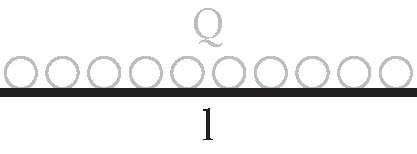
\includegraphics{bilder/kapitel/1/1.pdf}

2-dim: Fl�chenladungsdichte $\sigma = \dfrac{\mbox{Ladung auf der Fl�che}}{\mbox{Fl�che}}$\\
\fbox{$\sigma = \dfrac{Q}{A}$}\\
$[\sigma] = 1 \frac{As}{m^2} = \frac{Q}{m^2}$\\
%IMG-02.10.2008-physik-2
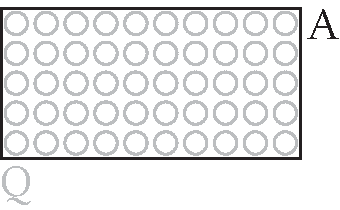
\includegraphics{bilder/kapitel/1/2.pdf}

3-dim: Raumladungsdichte $\rho = \dfrac{\mbox{Ladung im Raum}}{\mbox{Volumen des Raums}}$\\
\fbox{$\rho = \dfrac{Q}{V}$}\\
$[\rho] = 1 \frac{As}{m^3} = \frac{Q}{m^3}$\\
%IMG-02.10.2008-physik-3
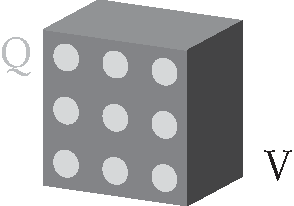
\includegraphics{bilder/kapitel/1/3.pdf}

\section{Die Coulombkraft}
\label{sec:DieCoulombkraft}
Aus der Beobachtung folgt:
zwischen geladenen Teilchen wirken Kr�fte diese werden im Allgemeinen als ''Coulombkr�fte'' bezeichnet. Sie wurde von ihrem Namensgeber C.A.Coulomb mithilfe der Torsionswage in Frankreich des 18. Jahrhunderts entdeckt.
\subsection{Definition}
Coulombkraft ist\dots
\begin{enumerate}
	\item proportional zum Produkt der Ladungen $Q_0 , Q_1$\\\textcircled{+}\textcircled{+}, \textcircled{-}\textcircled{-}:$~F>0$ $\Ra$ absto�end\\\textcircled{+}\textcircled{-}, \textcircled{-}\textcircled{+}:$~F<0$ $\Ra$ anziehend
	\item indirekt proportional zum Abstand $r^2$ der Ladungen
	\item parallel zu den Verbindungslinien der Ladungen\\
			IMG-06.10.2008-physik-1\\
			$\Rightarrow F_{01} \footnote{\mbox{(Die Kraft zwischen Ladung 0 und Ladung 1)}} ~ \dfrac{Q_0 \mal Q_1}{r_{01}^2}$
\end{enumerate}
\begin{description}
    \item[zu 3.)] IMG-06.10.2008-physik-2\\
						Ladung als Punktladungen idealisiert\\
						$\vec{F}_0 \vec{F}_1 =$ Ortsvektor\\
						$\vec{F}_0 = \vektor{x_0}{y_0}{z_0}, \vec{F}_1 = \vektor{x_1}{y_1}{z_1}$\\
						$\vec{r}_{01} = \vec{r}_0 - \vec{r}_0 = \vektor{x_0 - x_1}{y_0 - y_1}{z_0 - z_1} \Ra$ Richtung in der $\vec{F}_{01}$ wirkt.
\end{description}
\subsection{Abstand der Ladungen}
$r_{01} = \betrag{\vec{r}_{01}} = \sqrt{\left(x_0 - x_1\right)^2 + \left(y_0 - y_1\right)^2 + \left(z_0 - z_1\right)^2}$\\
Richtung:\\
Einheitsvektor (L�nge 1):\\
$\hat{\vec{r}}_{01} = \frac{\vec{r}_{01}}{\betrag{\vec{r}_{01}}}$ (Normierung)\\
\fbox{$\vec{F}_{01} = k \mal \dfrac{Q_0 \mal Q_1}{\betrag{\vec{r}_{01}}}^2 \mal \hat{\vec{r}}_{01}$}\\
Wobei $k$ eine proportionalit�tskonstante ist welche experimentell Bestimmt wird.
\[k = \frac{1}{4 \pi \epsilon_0}~~~~\epsilon_0 = \elefeldk\]
$\epsilon_0$ bezeichnet man als elektrische Feldkonstante.\\
\fbox{$\vec{F}_{01} = \frac{1}{4 \pi \epsilon_0} \mal \dfrac{Q_0 \mal Q_1}{\betrag{\vec{r}_{01}}}^2 \mal \hat{\vec{r}}_{01}$}\\
Einheit: $\left[ F_{01} \right] = 1N$

Beispiel: Buch S. 6\\
Gesucht: $\vec{F}_{01}$ von $Q_1$ auf $Q_0$
Gegeben:
\begin{alignat*}{2}
	Q_0 &= 1 \znr{-8} C, r_0 &&= \vektor{-3}{2}{1} \znr{-3} m\\
	Q_1 &= 3 \znr{-8} C, r_1 &&= \vektor{1}{-1}{1} \znr{-3} m\\
\end{alignat*}
\begin{alignat*}{2}
	\vec{r}_{01} &= \vec{r}_0 - \vec{r}_1 &&= \vektor{-4}{3}{0} \znr{-3} m\\
	\betrag{\vec{r}_{01}} &= \sqrt{(-4)^2 + (3)^2} \znr{-3} m &&= 5 \znr{-3} m\\
	\hat{\vec{r}}_{01} &= \frac{\vektor{-4}{3}{0} \znr{-3} m}{5 \znr{-3} m} &&= \vektor{-0,8}{0,6}{0}
\end{alignat*}
\begin{alignat*}{2}
	\vec{F}_{01} &= \frac{1}{4 \pi \epsilon_0} \mal \frac{Q_0 \mal Q_1}{\betrag{\vec{r}_{01}}}^2 \mal \hat{\vec{r}}_{01}\\
	&=\vec{F}_{01} = \frac{1}{4 \pi \epsilon_0} \mal \frac{1 \znr{-8} C \mal 3 \znr{-8} C}{\betrag{5 \znr{-3} m}^2} \mal \vektor{-0,8}{0,6}{0}\\
	&= \vektor{-86,3}{64,7}{0} \znr{-3} N\\
\betrag{\vec{F}_{01}} &= 107,9 mN
\end{alignat*}
Allgemein: Coulombkraft mehrerer ortsfester Ladungen $Q_i$ auf eine Ladung $q$
\renewcommand{\labelenumi}{\alph{enumi})}
\begin{enumerate}
	\item Berechnung jeder Kraft $\vec{F}_{q_i}$ seperat\[\vec{F}_{q_i} = \frac{1}{4 \pi \epsilon_0} \mal \dfrac{q \mal Q_i}{\betrag{\vec{F}_{q_i}}}^2 \mal \hat{\vec{F}}_{q_i}\]
	\item �berlagerung (Superposition) der Einzelkr�fte, daher vektorielle Addition\\\fbox{$\vec{F}_q = \sum_{i = 1}^n \vec{F}_{q_i}$}
\end{enumerate}
\renewcommand{\labelenumi}{\arabic{enumi})}
\section{Das elektrische Feld}
\subsection{Allgemeiner Feldbegriff}
Feld besteht aus:
\begin{itemize}
	\item Raum (leer oder stofferf�llt)
	\item Messbare physikalische Eigenschaften an jedem Raumpunkt\\$\Ra$ ''Feldgr��en'' (ortsabh�ngig)
\end{itemize}

Einteilung:
\begin{itemize}
	\item Skalarfelder\\nur Wert\\Beispiel: Temperaturfeld
	\item Vektorfeld\\Feldgr��e Betrag und Richtung\\Beispiel: elektrisches Feld oder Geschwindigkeitsfeld
\end{itemize}

Pfaddarstellung:\\
IMG-09.10.2008-physik-1\\

Feldliniendarstellung:\\
IMG-09.10.2008-physik-2\\

\begin{itemize}
	\item Pfeile zeigen in Richtung der Feldgr��e
	\item Tangenten an Feldlinien geben die Richtung der Feldgr��e an bestimmten Ort an
	\item Die Dichte gibt Betrag der Feldgr��e an
\end{itemize}

\begin{itemize}
	\item Quellenfelder\\Feldlinien haben Anfang (Quelle) und Ende (Ziel)\\z.B. elektrostatisches Feld\\elektrische Ladungen sind Quellen \textcircled{+} und Senken \textcircled{-} des elektrischen Feldes
	\item Wirbelfelder\\Feldlinien in sich geschlossen z.B. Magnetfeld
\end{itemize}

\section{\texorpdfstring{Die Elektrische Feldst�rke $\vec{\epsilon} (\vec{F})$}{Die Elektrische Feldst�rke Vektor Epsilon und Vektor F}}
Die elektrische Feldst�rke ist definiert als Coulombkraft die auf eine am Ort $\vec{F}$ befindlichen Probeladung $q$ wirken w�rde, bezogen auf die Probeladung.\\
allgemein beliebige Ladungsverteilung
\[\vec{F}_q (\vec{r}) = q \mal \frac{1}{4 \pi \epsilon_0} \sum_{i = 1}^n \frac{Q_i}{\betrag{F_{q_i}}^2 \mal \hat{\vec{F}}_{q_i}}\]
\fbox{$\vec{\epsilon} (\vec{r}) = \dfrac{\vec{F}_q}{q}$}\\
\begin{align*}
	\Ra~&\mbox{Kraft pro Ladungseinheit}\\
	&[\epsilon] = 1 \frac{N}{C} = 1 \frac{V}{m}\\
	\Ra &\vec{\epsilon} \mbox{ ist unabh�ngig vom Wert der Probeladung}\\
	\Ra &\vec{\epsilon} \mbox{ charakterisiert die Ladungsverteilung } Q_i\\
\end{align*}
$\vec{\epsilon}$ kann wie $\vec{F}_q$ durch Superposition errechnet werden\\
\fbox{$\vec{\epsilon} (\vec{r}) = \sum_{i = 1}^n \vec{e}_i (\vec{r})$}\\
IMG-09.10.2008-physik-3\\
Wenn $\vec{\epsilon} (\vec{r})$ bekannt, kann daraus Kraft auf eine Probeladung $p$ errechnet werden\\
\fbox{$\vec{F}_q = q \mal \vec{\epsilon} (\vec{r})$}\\
Analogie Gravitationsfeld:
\begin{align*}
	F &= m \mal g\\
	F &= m \mal \gamma \mal \frac{m^2}{r^2}
\end{align*}
Beispiel: Feld einer Punktladung $Q$
\[\vec{\epsilon} (\vec{r}) = \frac{\vec{F}_{qQ} (\vec{r})}{q}\]
\[\vec{F}_{qQ} (\vec{r}) = q \mal \frac{1}{4 \pi \epsilon_0} \frac{Q \mal q}{\betrag{F_{qQ}}^2 \mal \hat{\vec{r}}}\]
\[\vec{F}_{qQ} (\vec{r}) = q \mal \frac{1}{4 \pi \epsilon_0} \frac{Q}{\betrag{r}^2} \mal \hat{\vec{r}}\]
\[\Rightarrow \betrag{\vec{\epsilon}} ~ \frac{1}{r^2}\]
DIAG-09.10.2008-physik-1\\
$r \Ra 0$\\
math: $\epsilon \Ra \infty$\\
phys: keine Punktladung $\Ra r >0 \epsilon < \infty$

\subsection{Eigenschaften von Feldlinien}
\begin{itemize}
\item Bahn einer postiven Probeladung (Kraft auf Probeladung)
\item Tangenten $\rightarrow$ Richtung von $\vec{\epsilon}(\vec{F})$\\
		$\Ra \hat{\vec{\epsilon}}(\vec{F})$
\item Dichte $\rightarrow$ Betrag von $\vec{\epsilon}(\vec{F})$\\
		$\betrag{\vec{\epsilon}(\vec{F})}$
\item Beginnen bei \textcircled{+} (Quellen) enden bei \textcircled{-} (Senken)
\item IMG-13.10.2008-physik-1\\Feldlinien schneiden sich nie (sonst Kraftwirkung nicht eindeutig)
\item Itemoberfl�che\\IMG-13.10.2008-physik-2\\$\vec{\epsilon}(\vec{r})$ steht senkrecht auf Leiteroberfl�che, weil Ladungen im Leiter bewegen sich so lange bis $\vec{\epsilon}_r = 0$\\IMG-13.10.2008-physik-3
\end{itemize}
\section{Der elektrische Fluss}
allgemein Fluss:
\begin{itemize}
\item Eigenschaft eines Feldes
\item Durchsatz eines Feldes durch eine Fl�che
\end{itemize}
Beispiel: Volumenstrom\\
Geschwindikeitsfeld $\vec{v}$\\
IMG-13.10.2008-physik-4\\
Feldliniendichte $\propto \betrag{\vec{v}}$\\
Fluss/Durchstr�mungsrate\\
IMG-13.10.2008-physik-5
\begin{alignat*}{2}
	&v &&= \frac{s}{t}\\
	&s &&= v \mal t\\
	&\frac{v}{t} &&= A \mal v \mal t \mal \frac{1}{t}
\end{alignat*}
\fbox{$\phi = v \mal A$} $[\phi] = \frac{m^3}{s}$\\
Fl�che A:
$\vec{A}$\footnote{Ma� f�r Fl�cheninhalt}$ = \betrag{\vec{A}} \mal \hat{\vec{A}}$\footnote{Orientierung im Raum senkrechtzeichen auf Fl�chen}\\
IMG-13.10.2008-physik-6\\
Entscheidend f�r Fluss $\phi$ ist die senkrechte Projektion von $A$ auf Feld
\begin{alignat*}{2}
	\rightarrow \phi &= \betrag{\vec{v}} \mal \betrag{\vec{A}} \cosx{\mbox{\textcircled{-}}}\\
	& = \vec{v} \mal \vec{A}\\
	& = \vektor{v_x}{v_y}{v_z} \mal \vektor{A_x}{A_y}{A_z}\\
	& = v_x A_x + v_y A_y + v_z A_z
\end{alignat*}
$\rightarrow$ je gr��er die Feldlinienkonstante (hier $\betrag{\vec{v}}$) desto gr��er der Fluss $\phi$.
\subsection{\texorpdfstring{Elektrischer Fluss $\phi$}{Elektrischer Fluss Phi}}
Ma� f�r Feldlinien die Fl�che $A$ durchdringen
\subsection{Fluss durch beliebig geformte Fl�chen}
IMG-13.10.2008-physik-7\\
Fl�che in kleine Elemente $d \vec{A}_i$ zerlegen:\\
$\rightarrow \vec{\epsilon} = const$ durch $d \vec{A}_i$\\
$\rightarrow$ Fl�che $d \vec{A}_i$ plan\\
$\rightarrow d \phi_i$\footnote{Teilfluss: Fluss durch gesamte Fl�che $\vec{A}$ (Aufsummieren)}$= \vec{\epsilon} \mal d \vec{A}_i$\\
$\phi = \sum_{i = 1}^n d \phi_i = \sum_{i = 1}^n \vec{\epsilon} \mal d \vec{A}_i$\\
$d \vec{A}_1 \rightarrow 0$\footnote{Grenz�bergang : Summe $\rightarrow$ Integrale}$ = \iint \vec{\epsilon} \mal d \vec{A}_i$\\
$\iint , \int_A$ nennt man \quotate{Fl�chenintegral}\\
Berechnung ist oft kompliziert, aber durch geeignete Wahl der Fl�chengeometrie n.U. l�sbar
$\phi = \vec{\epsilon} \mal \vec{A}$\\
$\phi = \iint \vec{\epsilon} \mal d \vec{A}$\\
\renewcommand{\labelenumi}{Beispiel:}
\begin{enumerate}
\item elektrischer Fluss durch geschlossene Kugeloberfl�che\\
		IMG-16.10.2008-physik-1\\
		f�r jede Teilfl�che $d \vec{A}_i$ gilt:\\
		$\vec{e} \Vert d \vec{A}_i$
		\begin{align*}
			\phi &= \iint \vec{\epsilon} \mal d \vec{A} = \iint \epsilon d A\\
			&= \vec{\epsilon} \Vert d \vec{A} \rightarrow \cosx{\varphi} = 1
		\end{align*}
\end{enumerate}
\renewcommand{\labelenumi}{\arabic{enumi}.}
Weiterhin gilt:
\[\betrag{\vec{\epsilon}} (\vec{r}) = \frac{1}{4 \pi \epsilon_0} \mal \frac{Q}{r^2}\]
\[\rightarrow \betrag{\vec{\epsilon}} \mbox{ konstant auf Kugeloberfl�che weil $r =$ konstant auf Kugeloberfl�che}\]
\begin{align*}
	\phi &= \oiint \epsilon d A\\
		  &= \epsilon \oiint_A d A\\
		  &= \frac{Q}{4 \pi \epsilon_0 r^2}\\
		  &= \underbrace{\oiint_A i d A}_{\mbox{KOF} = 4 \pi r^2}\footnote{Kugeloberfl�che in Elemente zerlegt und aufsummiert}
\end{align*}
\fbox{$\phi = \dfrac{Q}{\epsilon_0}$}\\
$\phi$ durch geschlossene Fl�che (um Ladung herum) ist unabh�ngig vom Abstand $r$ (Ladung $\leftrightarrow$ Fl�che)\\
\begin{description}
\item[Allgemein:] gilt f�r jede beliebig geformte geschlossene Fl�che
\end{description}
\renewcommand{\labelenumi}{\arabic{enumi}.}
IMG-16.10.2008-physik-2\\
$\phi = \phi_i + \phi_R + \phi_v$
\begin{align*}
	\phi_i:~& \epsilon \mbox{ gro� }, A \mbox{ klein}\\
	\phi_R:~& \epsilon \mbox{ klein }, A \mbox{ gro�}\\
	\phi_v:~& \vec{A} \perp \vec{\epsilon} \rightarrow \varphi = 90\degree\\
			  & \rightarrow \vec{\epsilon} \mal \vec{A} = \epsilon A \underbrace{\cosx{\varphi}}_0 = 0\\
			  & \Ra \phi_v = 0
\end{align*}
\fbox{$\phi = \dfrac{Q}{\epsilon_0}$}
\section{Der Gau�sche Satz}
\subsection{Fluss durch geschlossene Fl�che}
IMG-16.10.2008-physik-3\\
keine Ladungen im Inneren!\\
$\phi = \phi_i + \phi_R + \phi_v$
\begin{description}
	\item[$\phi_i$:] IMG-16.10.2008-physik-4 $\phi = 180\degree$
			\begin{align*}
				\phi_i &= \iint_A \vec{\epsilon} \mal d \vec{A}_i = \iint_A \epsilon d A_i \cosx{\varphi}\\
			 	&= - \iint_{A_i} \epsilon d A_i = - \epsilon \iint_{A_i} d A_i = - \epsilon A_i
			\end{align*}
	\item[$\phi_R$:] IMG-16.10.2008-physik-5 $\phi = 0\degree$\\
			Analog zu $\phi_i$ folgt darau�:
		 	\[\Ra \iint_{A_R} \vec{\epsilon} \mal d \vec{A}_R = \epsilon A_R\]
	\item[$\phi_v$:] IMG-16.10.2008-physik-6 $\phi = 90\degree$\\
			Analog zu $\phi_i$ folgt darau�:
			\[\Ra \iint \vec{\epsilon} \mal d A_v = 0\]
\end{description}
Aus diesen einzellnen Formeln ergibt sich:
\begin{alignat*}{2}
	\phi &= \phi_i + \phi_R + \phi_v\\
	&= - \epsilon A_L + \epsilon A_R + 0\\
	&= - \epsilon A_i + \epsilon A_i = 0\\
	&\Ra \mbox{Ladungen au�erhalb geschlossener Fl�chen tragen nicht zum Fluss bei.}\\
	&\Ra \mbox{Nur Ladungen innerhalb dieser Fl�che bestimmen den Fluss}
\end{alignat*}
\fbox{$\phi = \oiint_A \vec{\epsilon} \mal d \vec{A} = \dfrac{1}{\epsilon_0} \sum_{i = 1}^n Q_i$} (Erste Maxwell Gleichung)
\subsection{Gau�sche Satz}
\begin{description}
\item[$\phi > 0$:] Quellen (\textcircled{+}) im Inneren von A\\
	IMG-16.10.2008-physik-7
\item[$\phi <0$:] Quellen (\textcircled{-}) im Inneren von A
\end{description}
%DIA-20.10.2008-phys-1
\begin{tikzpicture}
%Achsen mit Beschriftung
\draw [->] (-0.5,0) -- (10.5,0) node[anchor=north] {$r$};
\draw [->] (0,-0.5) -- (0,3.5) node[anchor=east] {$\rho = \dfrac{Q}{r}$};

%Kurve
\draw (5,0) -- (5,2.5);
\draw (0,0) .. controls (1.5,0.25) .. (2.5,1)
				.. controls (5,2) .. (7.5,1)
				.. controls (8.5,0.25) .. (10,0);
\end{tikzpicture}\\
Kontinuierliche Ladungsverteilung
\[\mbox{Raumladungsdichte: } \rho = \frac{\mbox{Ladung}}{\mbox{Volumen}} = \frac{D}{V}\]
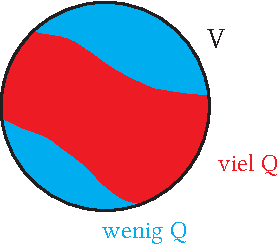
\includegraphics{bilder/kapitel/1/4.pdf}\\%IMG-20.10.2008-phys-1
$Q = \iiint_V \underbrace{\rho}_{\mbox{nicht konstant}} \mal d V \leftarrow$ Ladungen im inneren von $V$\\
\fbox{$\oiint_A \vec{\epsilon} \mal d \vec{A} = \dfrac{1}{\epsilon_0} \mal \iiint_V \rho \mal d V$}
\[\oiint_A \vec{\epsilon} \mal d \vec{A} \mbox{ ist der Fluss durch die geschlossene Fl�che $A$}\]
\[\frac{1}{\epsilon_0} \mal \iiint_V \rho \mal d V \mbox{ ist die Ladung im Inneren von $V$ (bzw. $A$)}\]
$\vec{F} = q \mal \vec{\epsilon}$\\
Der Gau�sche Satz ist eine andere Formulierung des Coulombgesetzes.\\
Er erleichtert die Berechung von elektrischen Feldern mit einfacher und symmetrischer Anordnung.\\
Die geschlossene Fl�che $A$ muss der Geometrie des Elektrischen Feldes angepasst werden.
\begin{itemize}
\item $\vec{\epsilon} \Vert d \vec{A} \Rightarrow \vec{\epsilon} \circ d \vec{A} = \betrag{\vec{\epsilon}} \betrag{\vec{A}}$
\item $\betrag{\epsilon} =$ konstant auf Fl�che $A \Rightarrow \oiint_A \epsilon \mal d A = \epsilon \oiint_A d A$
\item $\iint_A d A = A \mbox{ (Die Oberfl�che der Fl�che $A$}$
\end{itemize}
\subsection{Geladene Isolatorkugel}
\begin{description}
\item[Isolator:] Nichtleiter\\
		$\Ra$ Ladungen sind unbeweglich
		$\Ra$ Gleichm��ig �ber Volumen Verteilt
\end{description}
IMG-23.10.2008-physik-1\\
Gesammtes $\epsilon$ innen und au�en
\renewcommand{\labelenumi}{\alph{enumi})}
\begin{enumerate}
\item Au�enraum\\
		wie 1.6.1 a) (leitende Kugel)
		\[\epsilon = \frac{Q}{4 \pi \mal \epsilon_0} \frac{1}{r^2}\]
\item Innenraum\\
		Gau�fl�che $\equals$ Kugeloberfl�che mit Radius $r < R$\\
		Ladungen innerhalb Gau�fl�che
		\[Q = \rho V_{GF} = \rho \frac{4}{3} \pi r^3\]
		$\oiint_A \vec{\epsilon} = d \vec{A} = \epsilon \oiint_A d A = \epsilon 4 \pi r^2 = \frac{Q}{\epsilon_0} = \rho \frac{4}{3} \pi r^3 \frac{1}{\epsilon_0}$\\
		$\Ra$ \fbox{$\epsilon = \frac{\rho 4 \pi r^3}{\epsilon_0 3 \mal 4 \pi r^2} = \frac{1}{3} \frac{\rho}{\epsilon_0} \mal r$}
		\begin{tikzpicture}
		%Achsen mit Beschriftung
		\draw [->] (-0.5,0) -- (10.5,0) node[anchor=north] {$r$};
		\draw [->] (0,-0.5) -- (0,3.5) node[anchor=east] {$\epsilon$};

		%Kurve
		\draw[dashed] node[anchor=east]{$\epsilon_{Max}$}(0,2.5) -- (3,2.5);
		\draw node [anchor=south]{$\propto r$} (0,0) -- (3,2.5);
		\draw (3,2.5) .. controls (4.5,0.5) .. (9,0) node[anchor=south] {$\propto \dfrac{1}{r^2}$};
		\draw node [anchor=north]{$R$} (3,-0.5) -- (3,0.5);
		%\draw circle (3,2.5);
		\end{tikzpicture}\\
		\begin{alignat*}{2}
			\mbox{aus a) folgt }\epsilon_{\mbox{Max}} &= \frac{Q}{4 \pi \epsilon_0 R^2}\\
			\mbox{aus b) folgt }\epsilon_{\mbox{Max}} &= \frac{1 \rho \mal R}{3 \epsilon_0}\\
			&=\frac{Q 3 R}{3 \epsilon_0 \mal 4 \pi R^2}
		\end{alignat*}
		$\Ra$ im Au�enseiter\\
		$\epsilon$-Feldverlauf derselbe bei Punktladung, leitender Kugel und Isolatorkugel
\end{enumerate}
\renewcommand{\labelenumi}{\arabic{enumi}.}
\subsection{Lange gerader Leiterdraht}
IMG-23.10.2008-phys-4\\
\begin{tikzpicture}
\draw (0,0) -- (2,2);
%\draw klammer (0,0) -- (2,2); mit nem L unter der Klammer
%links davon Radius R \\ L >> R
\end{tikzpicture}
gleichm��ige Ladungsverteilung\\
\[\rightarrow \mbox{ Ladungsdichte } \lambda = \frac{Q}{L} = \mbox{ const}\]
IMG-23.10.2008-phys-2\\
Radialsymmetrie\\$\Ra$ jede Oberfl�che gleich\\
$\Ra$ GF: Zylinder mit Radius $r$ wobei Deckfl�che vernachl�ssigbar ist\\
$\rightarrow$ betrachte Mangelfl�che\\
\[\oiint_A \vec{\epsilon} \circ d \vec{A} \underbrace{=}{\vec{\epsilon} \Vert \vec{A}} \epsilon \oiint_A d A = \epsilon \underbrace{2 \pi r L}_{\mbox{Mantelfl�che Zylinder}} \underbrace{=}_{GS} \frac{Q}{\epsilon_0} \underbrace{=}_{\lambda = \frac{Q}{L}} \frac{\lambda L}{\epsilon_0}\]
\[\Ra \epsilon = \frac{\lambda L}{\epsilon_0 2 \pi r L^2}\]
$\Ra$ \fbox{$\epsilon (r) = \frac{1}{2\pi} \mal \frac{\lambda}{\epsilon_0} \mal \frac{1}{r}$}\\
\subsection{Ebene, geladene Leiterplatte}
IMG-23.10.2008-phys-6\\
homogen geladen
\[\mbox{Fl�chenladungsdichte } \sigma = \frac{Q}{A} = \mbox{ const}\]
IMG-23.10.2008-phys-7\\
IMG-23.10.2008-phys-8\\
GF: Quader mit Grundfl�che a\\$\rightarrow$ betrachte Deckfl�che
\[\phi = \epsilon_{\mbox{oben}} \mal a + \epsilon{\mbox{unten}} \mal a \underbrace{=}{\epsilon_{\mbox{oben}} = \epsilon_{\mbox{unten}}} 2 \epsilon \mal a \underbrace{=}{as} = \frac{Q}{\epsilon_0}\]
\[2 \epsilon a = \frac{\sigma a}{\epsilon_0}\]
$\Ra$ \fbox{$\epsilon = \frac{\sigma}{2 \epsilon_0} = \mbox{ const}$}\\
IMG-23.10.2008-phys-9

\section{Berechnung einfacher elektrischer Felder}
\subsection{Geladene, leitende Kugeln}
Die leitende Kugel mit dem Radius $R$ und mit der Ladung $Q$\\
Leitend hei�t, dass die Ladungen sich frei bewegen k�nnen. Durch die absto�enden Coulombkr�fte versuchen die Ladungen sich soweit wie m�glich voneinander zu entfernen.\\
$\longrightarrow$ gleichm��ige Verteilung der Ladungen an der Oberfl�che.\\
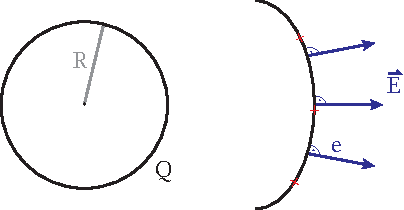
\includegraphics{bilder/kapitel/1/5.pdf}\\%IMG-20.10.2008-phys-2
Feldlinien treten senkrecht aus der Oberfl�che aus.\\
$\longrightarrow$ Kugelsymmetrie\\
$\longrightarrow$ $\betrag{\vec{\epsilon}} =$ konstant auf Kugeloberfl�che
\renewcommand{\labelenumi}{\alph{enumi})}
\begin{enumerate}
\item Au�enraum\\
		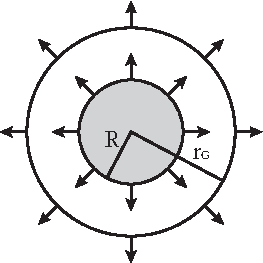
\includegraphics{bilder/kapitel/1/6.pdf}\\%IMG-20.10.2008-phys-3
		Gau�fl�che $\rightarrow$ Kugeloberfl�che mit Radius $r > R$\\
		\begin{alignat*}{2}
		&\oiint_A \vec{\epsilon} \mal d \vec{A} = \frac{1}{\epsilon_0} Q_{\mbox{eingeschlossen}}\\
		\underbrace{=}_{\vec{\epsilon} \Vert d \vec{A}} &\oiint_A \epsilon \mal d A \underbrace{=}_{\betrag{\epsilon} = \mbox{ konstant auf KOF}} \epsilon \iint_A d A \underbrace{=}_{\mbox{KOF}} \epsilon 4 \pi r^2 = \frac{Q}{\epsilon_0}
		\end{alignat*}
		$\Rightarrow$ \fbox{$\epsilon = \dfrac{Q}{4 \pi \epsilon_0 \mal r^2}$}\\
		vergleichen: Ladung $Q$ im Mittelpunkt konzentriert
\item Innenraum\\
		Gau�fl�che $\rightarrow$ Kugeloberfl�che $r < R$\\
		$\oiint_A \vec{\epsilon} \mal d \vec{A} = \frac{1}{\epsilon_0} Q_{\mbox{eingeschlossen}} = 0$\\
		Analog zu a) $\Rightarrow$ $\epsilon 4 \pi r^2 = 0$\\
		$\Rightarrow$ \fbox{$\epsilon = 0$}\\
		$\Rightarrow$ Inneres von leitf�higen K�rpern ist Ladungsfrei\\
		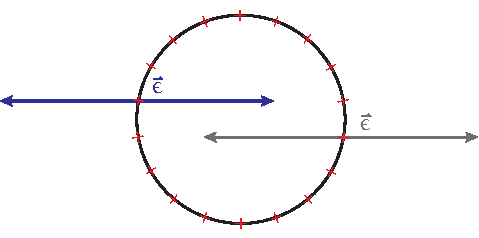
\includegraphics{bilder/kapitel/1/7.pdf}\\%IMG-20.10.2008-phys-4
		%DIA-20.10.2008-phys-2
\begin{tikzpicture}
		%Achsen mit Beschriftung
		\draw [->] (-0.5,0) -- (10.5,0) node[anchor=north] {$r$};
		\draw [->] (0,-0.5) -- (0,3.5) node[anchor=east] {$\epsilon = \dfrac{Q}{4 \pi \epsilon_0 R^2}$};

		%Kurve
		\draw[dashed] (0,2.5) -- (3,2.5);
		\draw (3,0) -- (3,2.5);
		\draw (3,2.5) .. controls (4.5,0.5) .. (9,0) node[anchor=south] {$\propto \dfrac{1}{r^2}$};

		%Beschriftung
		\draw [<-] (0,-0.5) -- (1.5,-0.5) node[anchor=north] {innen};
		\draw [->] (1.5,-0.5) -- (3,-0.5);
		\draw [<-] (3,-0.5) -- (6,-0.5) node[anchor=north] {au�en};
		\draw [->] (6,-0.5) -- (9,-0.5);
		\draw [dashed] (9,-0.5) -- (9,0);
		\end{tikzpicture}\\
		$\epsilon = \frac{Q}{4 \pi \epsilon_0} \mal \frac{1}{r}$
\end{enumerate}
Schlussfolgerung:
\begin{itemize}
\item Das innere von Leitern ist immer feldfrei (Farad�ischer K�fig)
\item $\epsilon$ an leitender Oberfl�che:\\
		$\epsilon \propto \frac{1}{R^2}$ wobei $R$ der Kr�mmungsradius ist\\
		$\rightarrow$ kleine Kr�mmungsradien (Spitzen)
		$\rightarrow$ hohe Feldst�rken
\item Ladungen nur an Leiteroberfl�chen\\
		Fl�chenladungsdichte: $\sigma = \frac{Q}{A}$\\
		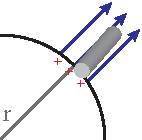
\includegraphics{bilder/kapitel/1/8.pdf}\\%IMG-20.10.2008-phys-5
		$\phi = \oiint_A \vec{\epsilon} \mal d \vec{A} = \frac{1}{\epsilon_0} \iiint_V \rho \mal d V$\\
		$~~~  = \frac{1}{\epsilon_0} \iint_A \sigma \mal d A$\\
		$\epsilon \mal d A = \frac{\sigma}{\epsilon_0} \mal d A$\\
		$\frac{Q}{A}$ = \fbox{$\sigma = \epsilon_0 \mal \epsilon_{\mbox{oberfl�che}}$}\\
		$\longrightarrow$ Elelektrische Feld an der Oberfl�che $\propto$ Fl�chenladungsdichte
\end{itemize}
\renewcommand{\labelenumi}{\arabic{enumi}.}

%\chapter{Potentiale und Spannungen}
\label{sec:PotentialeundSpannungen-2}
\section{Elektrische Potential}
Analog: Gravitationsfeld\\
IMG-27.10.2008-phys-1\\
Mechanische arbeit $W$ verrichten um Masse $m$ auf H�he $h$ zu heben!
\[W = m \mal g \mal h = m \mal g \mal s \mal \cosx{\alpha}\]
$\rightarrow$ Arbeit wird gespeichert als potentielle Energie\\
IMG-27.10.2008-phys-2\\
$W = F_{\mbox{mech}} \mal s_{\Vert} = F_{\mbox{mech}} \mal s \mal \cosx{\alpha}$\\
\fbox{$W = \vec{F}_{\mbox{mech}} \circ \vec{s}$} $[W] = Nm = J \mbox{ (Joule)}$\\
\subsection{Kraft konstant entlang des Weges}
IMG-27.10.2008-phys-3\\
$\Rightarrow W \equals $ Fl�che unter der Kurve\\
$N = \frac{kg \mal m}{s^2}$
$W_{AB} = \Delta \epsilon_{pot}$\\
$W_{AB} = -q \int_A^B \vec{\epsilon} \circ d \vec{r}$\\
Bewegung $\Vert$ Feldlinien\\
Bewegung $\perp$ Feldlinien: $\omega = 0$\\
$\ra$ jeden Raumpunkt kann ein ''Potential'' $\varphi$ zugewiesen werden.
$\ra$ abh�ngig vom Abstand $r$ zur felderzeugenden Ladung
$\ra$ Definition Potential $\varphi_a$
Pro Ladung $q$ zu verrichtende Arbeit um diese vom Bezugspunkt $r = \infty$ (dort $\epsilon = 0$) zum Punkt $A(r = r_A)$ zu bewegen.
\fbox{$\varphi_A := \dfrac{\omega_{\infty A}}{q}$}\\
$\ra$ Eigenschaft des elektrischen Feldes Ladungen zu bewegen\\
$\ra$ unabh�ngig von der PRobeladung $q$\\
$[\varphi] = \frac{Nm}{C} = \frac{J}{As} \frac{VAs}{As} = V$ (''Volt'')\\
$J = VAs = Nm$
$\ra V = \frac{Nm}{As} = \betrag{\betrag{\frac{kg m^2}{s^2 As}}} = \frac{kg m^2}{s^3 A}$\\
f�r Punktladung (s.o.)\\
$\varphi_A (r_A) = \frac{\omega_{\infty A}}{q} = \frac{q Q}{q 4 \pi \epsilon_0} \mal \left(\frac{1}{r_A} - \underbrace{\frac{1}{\infty}}_{=0} \right)$\\
\fbox{$\varphi_A = \frac{Q}{4 \pi \epsilon_0} \frac{1}{r_A}$}\\
nicht verwechseln!\\
potentielle Energie = Arbeit an Ladung verrichtet\\
Potential = $\frac{\mbox{Arbeit}}{\mbox{Ladung}}$\\
Fl�che konstanen Potential:
\subsection{�quipotentialfl�chen}
Eigenschaften:
\begin{itemize}
\item $\varphi =$ konstant
\item Bewegung auf dieser Fl�che\\
		keine arbeit zu verrichten
\item �quipotentialfl�chen $\perp$ Feldlinien\\
		$\ra$ Leiteroberfl�chen sind �quipotentialfl�chen\\
		IMG-30.10.2008-phys-1
		IMG-30.10.2008-phys-2
\end{itemize}
\subsection{\texorpdfstring{Zusammenhang Potential-$\epsilon$-Feld}{Zusammenhang Potential-Epsilon-Feld}}
$\varphi_A = \frac{\omega_{\infty A}}{q} = - \frac{q}{q} \int \vec{\epsilon} \circ d \vec{r}$\\
$\underbrace{=}_{\vec{\epsilon} \Vert d \vec{r}} - \int \epsilon dr$\\
$\Ra \varphi (r) = - \int \epsilon dr \left\| \mal \frac{d}{dr} \right.$\\
$\frac{d \varphi}{d r} = - \epsilon$\\
DIA-30.10.2008-phys-1\\
$\Ra$ \fbox{$\epsilon = - \frac{d \varphi}{dr}$}\\
$\ra \betrag{\vec{\epsilon}}$ proportional zur �nderung des Potentials\\
$\longrightarrow \hat{\vec{\epsilon}}$ zeigt entgegen der Richtung der (st�rksten) �nderund des Potentials
\section{Elektrische Spannung}
\label{sec:ElektrischeSpannug}
Zur ANgabe von Potentialen beziehungsweise potentieller Energien ist immer ein Bezugspunkt n�tig\\
F�r elektrisches Potential: Bezugspunkt im Unendlichen $\ra \varphi_{\infty} = 0$\\
\subsection{Potentialdifferenz}
Meistens nur dir Potentialdifferenz relevant in der Physik\\
\fbox{elektrische Potentialdifferenz = Spannung}\\
$U_{AB}$ = die Spannung zwischen den Punkten $A$ und $B$\\
$U_{AB} = \varphi_B - \varphi_A = \varphi_{\infty B} - \varphi_{\infty A} = \frac{\omega_{\infty B}}{q} - \frac{\omega_{\infty A}}{q}$\\
IMG-30.10.2008-phys-3\\
$W_{\infty A} + W_{AB} - W_{\infty B} = 0$\\
$\Ra W_{\infty B} - W_{\infty A} = W_{AB}$\\
$\Ra$ \fbox{$U_{AB} = \dfrac{W_{AB}}{q} = - \int_A^B \vec{\epsilon} \circ d \vec{r}$} $[U] = [\varphi] = V$\\
$\ra$ Arbeit $W_{AB}$ ist unabh�ngig vom gew�hlten Weg von $A$ nach $B$\\
$\ra$ Spannung $U_{AB}$ ist unabh�ngig vom gew�hlten Weg von $A$ nach $B$\\
DIA-30.10.2008-phys-2\\
Ges: $U_{AB}$\\
sinnvolle Zerlegung des Weges parallel zu Feldlinien ($A \ra P$), und entlang von �quipotentialfl�che ($P \ra B$)\\
$U_{PB} = \varphi_B - \varphi_P = 0$\\
$\varphi_A =\frac{W_{\infty A}}{q}$\\
$\ra$ Fl�chen konstanter Potentiale\\
IMG-02.11.2008-phys-1\\
$U_{AB} ) \varphi_B - \varphi_A$\\
Beispiel:\\
IMG-02.11.2008-phys-2\\
$U_{AB} = - \int_A^B \vec{\epsilon} \mal d \vec{r}$\\
$U_{PB} = \varphi_B - \varphi_P \underbrace{=}_{\mbox{�quipotentialfl�che}_p: \varphi_P = \varphi_B} 0$
$U_{AP} = - \int_A^P \vec{\epsilon} \mal d \vec{r} \underbrace{=}_{\vec{\epsilon} \Vert d \vec{r}} - \int_A^P \epsilon (r) dr =$\\
$\epsilon (r) = \frac{1}{4 \pi \epsilon_0} \frac{Q}{r^2} \ra$ abh�ngig von $r$!\\
$U_{AP} = - \int_A^P \frac{Q}{4 \pi \epsilon_0} \frac{1}{r^2} dr = \int r^{-2} dr = -1 r^{-1}$\\
$=- \frac{Q}{4 \pi \epsilon_0} \int_A^P \frac{1}{r^2} dr = - \frac{Q}{4 \pi \epsilon_0} \left[-\frac{1}{r}\right]_{r_A}^{r_P}$\\
$= + \frac{Q}{4 \pi \epsilon_0} \left( \frac{1}{r_P} - \frac{1}{r_A} \right)$\\
$U_{AB} = U_{AP} + \underbrace{U_{PB}}_{= 0} = \frac{Q}{4 \pi \epsilon_0} \left( \frac{1}{r_B} - \frac{1}{r_A} \right)$\\
$W_{AB} = U_{AB} q$
\section{Influenz}
Leiter im elektrostaischem Feld\\
$\ra$ Ladungen sind innerhalb frei beweglich\\
$\longrightarrow$ Verschreibung von Ladungen durch �u�eres elektrisches Feld\\
IMG-02.11.2008-phys-3\\
Feldlinien $\perp$ Leiteroberfl�che (1.3)\\
$\leftrightarrow$ Ladungen bewegen sich solange, bis
\[\vec{\epsilon}_{\Vert} \propto \vec{F}_{\Vert} = 0\]
$\Ra$ Leiteroberfl�chen sind �quipotentialfl�chen\\
IMG-02.11.2008-phys-4\\
Beispiel:\\
Neutrales Leiterst�ck im Feld einer Punktladung\\
IMG-02.11.2008-phys-5\\
Feld im Leiterinneren
\[\vec{\epsilon}_{inners} = \vec{\epsilon}_a + \vec{\epsilon}_{\infty} = 0 \]
$\Ra$ Leiterinneres ist immer feldfrei (siehe 1.6)\\
\subsection{Faradayscher K�fig (ungeerdet)}
\renewcommand{\labelenumi}{\alph{enumi})}
\begin{enumerate}
\item �u�eres Feld\\
		IMG-02.11.2008-phys-6\\
		$\vec{\epsilon}_{innen} = \vec{\epsilon}_a + \vec{\epsilon}_{\infty} = 0$\\
		\begin{itemize}
		\item �u�eres Feld kann in K�figinneres nicht eindringen
		\item H�lle $\equals$ �quipotentialfl�chen
		\end{itemize}
\item inneres Feld\\
		IMG-02.11.2008-phys-7\\
		IMG-02.11.2008-phys-8\\
\end{enumerate}
\renewcommand{\labelenumi}{\arabic{enumi}.}

%\chapter{Der Kondensator}
Aufbau zwei Leiterfl�chen durch Isolator (sogenanntes Dielektrikum) getrennt\\
%IMG-06.11.2008-physik-1
\begin{tikzpicture}
	\draw (0,0) -- (2,0);
	\draw (0,1) -- (2,1);
	\draw (1,1.5) -- (1,1);
	\draw (1,-0.5) -- (1,0);
%TODO	\draw[decoration=crosses] (0,-0.25) -- (0.9,-0.25);
\end{tikzpicture}
\renewcommand{\labelitemi}{$\rightarrow$}
\begin{itemize}
\item Speicherung von Ladungen\footnote{lateinisch condensus: dicht gedr�ngt} und somit Energie
\item passives Standartbauteil der Elektronik
\end{itemize}
\renewcommand{\labelitemi}{$\bullet$}
Anwendung:
\begin{itemize}
\item Ladungsspeicher (DRAM)
\item Energiespeicher (Blitzger�t)
\item Gl�ttung von Wechselspannung (Netzteil)
\item Frequenz beziehungsweise zeitabh�ngige Bauteil in Filter, Schwingkreise, Verz�gerungsglieder (Hochpass, Tiefpass, Senderabstimmung)
\end{itemize}
Schaltzeigen:
%IMG-06.11.2008-physik-2
\begin{tikzpicture}

\end{tikzpicture}
\section{\texorpdfstring{Die Kapazit�t $C$}{Die Kapazit�t C}}
\renewcommand{\labelitemi}{$\rightarrow$}
\begin{itemize}
\item Ma� f�r F�higkeit eines Kondensators Ladungen zu speichern
\end{itemize}
\renewcommand{\labelitemi}{$\bullet$}

\renewcommand{\labelenumi}{\alph{enumi})}
\begin{enumerate}
\item Kugelkondensator\\
		IMG-06.11.2008-physik-2
		\renewcommand{\labelitemi}{$\rightarrow$}
		\begin{itemize}
		\item Hohlkugel (leitf�hig) um leitf�hige Kugel\\
				Kugelfl�chen: Leiteroberfl�chen\\
				$\hookrightarrow$ �quipotentialfl�chen
		\end{itemize}
		\renewcommand{\labelitemi}{$\bullet$}
		\begin{align*}
			\Ra &\varphi_i = \mbox{ const }, \varphi_a = \mbox{ const}\\
			&\mbox{Spannung zwischen Kugelfl�chen}\\
			&U_{ai} = \varphi_i - \varphi_a = - \int_{r_a}^{r_i} \vec{\epsilon} \circ d \vec{r} \mbox{ vgl. \ref{sec:ElektrischeSpannug}}\\
			&U = \underbrace{\frac{1}{4 \pi \epsilon_0} \left(\frac{1}{r_i} - \frac{1}{r_a}\right)}_{\mbox{konstante Geometriegr��e} \ra C} Q\\
			&U \propto Q
		\end{align*}
		\fbox{$Q = C \mal U$}
		\renewcommand{\labelitemi}{$\rightarrow$}
		\begin{itemize}
		\item Proportionalit�tskonstante ''Kapazit�t'' $C$ gilt f�r beliebige Geometrie
		\item F�higkeit (einer geometrischen Anordnung) bei Spannung $U$ eine Ladung $Q$ zu speichern
		\end{itemize}
		\renewcommand{\labelitemi}{$\bullet$}
		$[C] = \dfrac{[Q]}{[U]} = \dfrac{C}{V} = \dfrac{A}{As} = F$ ''Farad''

\item IMG-06.11.2008-physik-4\\
		N�herung zweier konzentrischer Kugeln (wie $\omega$) mit\\
		$r_a = r_i + d, d \ll r_i$\\
		$\begin{array}{ll}
		C &= 4 \pi \epsilon_0 \left(\frac{r_i r_a}{r_a - r_i}\right) = 4 \pi \epsilon_0 \left(\frac{r_i (r_i + d)}{r_i + d - r_i}\right)\\
		  &= 4 \pi \epsilon_0 \left(\frac{r_i^2}{d}\right) = \epsilon_0 \left(\frac{2 \pi r_i^2}{d}\right)
		\end{array}$\\
		$4 \pi r_i^2 = \mbox{Kugeloberfl�che } A$\\
		$\Ra$ \fbox{$C = \epsilon_0 \dfrac{A}{d}$} mit
		\begin{tabular}{ll}
		$A$&: Plattenfl�che\\
		$d$&: Plattenabstand
		\end{tabular}
		\renewcommand{\labelitemi}{$\rightarrow$}
		\begin{itemize}
		\item IMG-06.11.2008-physik-5\\
				Beispiel: Plattenkondensator mit $C = 1 F$\\
				\[\begin{array}{lll}
					\mbox{Geg: } &C &= 1 F\\
					&d &= 1mm\\
					\mbox{Ges: } &A&\\
				\end{array}\]
				\[\begin{array}{lll}
					\mbox{L�sung: } &C &= \epsilon_0 \frac{A}{d}\\
					&A &= \frac{C \mal d}{\epsilon} = \frac{1 \mal 1 \znr{-3}}{8,85 \znr{-12}} \frac{As m Vm}{V As}\\
					&&= 113 km^2
				\end{array}\]
				\renewcommand{\labelitemii}{$\rightarrow$}
				\begin{itemize}
				\item Quadrat mit Seitenl�nge $10,63 km$
				\item $1F$ riesige Kapazit�t
				\end{itemize}
				\renewcommand{\labelitemii}{\textendash}
		\end{itemize}
		\renewcommand{\labelitemi}{$\bullet$}
\end{enumerate}
\renewcommand{\labelenumi}{\arabic{enumi}.}
\subsection{Elektrisches Feld}
IMG-06.11.2008-physik-6 IMG-06.11.2008-physik-7\\
$\epsilon = 2 \mal \epsilon_{\mbox{Einzelplatte}} = 2 \dfrac{\sigma}{2 \epsilon_0} = \dfrac{\sigma}{2 \epsilon_0} = \mbox{const}$
\renewcommand{\labelitemi}{$\Rightarrow$}
\begin{itemize}
\item homogenes elektrisches Feld zwischen Platten im Innenraum (Randeffekte vernachl�ssigt)
\end{itemize}
\renewcommand{\labelitemi}{$\bullet$}
\[\begin{array}{ll}
	U &= \int \epsilon dr = \frac{Q}{C}\\
	&= \epsilon \intx{0}{d}{dr}\\
	&= \epsilon d = U\\
\end{array}\]
\[\Ra \epsilon = \frac{U}{d}\]
IMG-10.11.2008-phys-1\\
$Q = C \mal U$\\
Plattenkondensator:
\begin{alignat*}{2}
	C &= \epsilon_r \epsilon_0 \mal \frac{A}{d}\\
	\epsilon &= \frac{U}{d} 
\end{alignat*}

\section{Gespeicherte Energie im Kondensator}
Laden eines Kondensators bedeutet Ladungstrennung $\ra$ Energieaufwand (Arbeit). Diese Arbeit wird als elektrische Energiedichte in elektrischem Feld gespeichert.
\[U = \frac{W_{el}}{Q}\]
\[W_{el} \mbox{ ist die geleistete Arbeit zum Laden}\]
Um infinitesimal kleine Ladungen $dQ$ von der positiven zur negativen Platte zu verschieben ist Arbeit $dW$ notwendig.
\[dW = \underbrace{U}_{U = U (Q)} dQ \underbrace{=}_{U = \frac{Q}{C}} \frac{Q}{C} dQ\]
\[W = \intx{0}{Q}{dW} = \intx{0}{Q}{\frac{1}{C} Q' d Q'} = \frac{1}{C} \intx{0}{Q}{Q' d Q'}\]
\begin{alignat*}{2}
	W &= \frac{1}{C} \left[\frac{1}{2} Q'^2\right]^Q_0 = \frac{1}{C} \mal \frac{1}{2} \mal \left(Q^2 - 0\right)\\
	&= \frac{Q^2}{2C} \underbrace{=}{Q = C \mal U} \frac{C^2 U^2}{2l}
\end{alignat*}
\fbox{$\frac{1}{2} C U^2 = \frac{1}{2} Q U = W_{el}$}\\
gilt f�r beliebige Geometrie, da $W = Q \mal U$ und $Q = C \mal U$ allgemein g�ltig sind.

\section{Kraft zwischen Kondensatorplatten}
IMG-10.11.2008-phys-2\\
Ladungen unterschiedlichen Typs ziehen sich an (vgl. \ref{sec:DieCoulombkraft}\\
$\ra$ Kondensatorplatten ziehen sich an\\
Arbeit $dW$ um eine Platte in $dr$ zu verschieben (Platte bewegen hei�t Ladungen im elektrischen Feld bewegen $\ra$ Arbeit)
\[\begin{array}{lll}
	&\mbox{Arbeit } &= \mbox{ Kraft } \mal \mbox{ Weg}\\
	&dW &= F dr\\
	\Ra & F &= \frac{dW}{dr} = \frac{d}{dr} \left(\frac{1}{2} Q U \right) = \frac{1}{2} Q \frac{dU}{dr}
\end{array}\]
\fbox{$F = \frac{1}{2} Q \epsilon$}\\
\textalign{Anwendung:}{elektrostatische Aktoren (Antriebe) in der Mikrosystemtechnik}
IMG-10.11.2008-phys-3 IMG-10.11.2008-phys-4
\textalign{Beispiel:}{Plattenkondensator\\
$C = 200pF$\\
$A = 0,25 m^2, Q = 2 u C$\\
\textalign{Gesucht:}{Plattenabstand $d$, Kraft zwischen Platten $F$}
\textalign{L�sung:}{$C = \epsilon_0 \frac{A}{d}$
\[\begin{array}{lll}
	\Ra & d &= \epsilon_0 \frac{A}{C} = \frac{8,85 \znr{-12} \mal 0,25}{200 \znr{-12}} \frac{As \mal m^2}{Vm As}\\
	&&= 0,011m = 1,1cm\\
	F &&= \frac{1}{2} Q \epsilon = \frac{1}{2} Q \frac{U}{d} = \frac{1}{2} Q \frac{Q}{C d}\\
	&&= \frac{\left(2 \znr{-9}\right)^2}{2 \mal 200 \znr{-12} 1,1 \znr{-2}} \frac{A^2 s^2 V}{As m} = 9,1 \znr{-7} \frac{J}{m} = 910 nN
\end{array}\]}}

\section{Kondensatorschaltungen}
\subsection{Parallelschaltung}
\textfakealign{Gesucht:}{IMG-10.11.2008-phys-5}
\textalign{Gesucht:}{$C$ Gesamtkapazit�t
\begin{alignat*}{2}
	&Q = Q_1 + Q_2~~U = U_1 = U_2\\
	&Q = CU
	\Ra&CU = C_1 U_1 + C_2 U_2\\
	&CU = C_1 U + C_2 U = U \left( C_1 + C_2 \right)
\end{alignat*}
$\Ra$ \fbox{$C = C_1 + C_2$}}

\textalign{Allgemein:}{\fbox{$C = \sumx{i = 1}{N}{C_i}$}\\
IMG-10.11.2008-phys-6\\
\textalign{$\Ra$}{Parallelschaltung entspricht Vergr��erung der Plattenfl�chen}

\textalign{Beispiel:}{$C_1$ auf $U_1$ laden, IMG-10.11.2008-phys-7\\
dann ungeladene $C_2$ parallelschalten (Schalter schlie�en)\\
\textalign{Gesucht:}{$U$ nach Ende des Umladevorgangs}

\textalign{L�sung:}{$Q_1 = C_1 \mal U_1 = \mbox{ const}$\\
$\underbrace{C_1 U_1}_{\mbox{vorher}} = \underbrace{\left(C_1 + C_2\right)}_{\mbox{nachher}} U$\\
$U = \frac{C_1}{C_1 + C_2} U_1$
\begin{alignat*}{2}
\Ra &U &&= \frac{C_1}{2 C_1} U_1\\
&&= \frac{1}{2} U_1
\end{alignat*}}}}

\subsection{Reihenschaltung}
IMG-10.11.2008-phys-8 	IMG-10.11.2008-phys-9 $\Ra$ Influenz\\
$Q_1 = Q_2 = Q$			$U = U_1 + U_2$ %align%
\begin{alignat*}{2}
	U = \frac{Q}{C} \Ra &\frac{Q_1}{C_1} + \frac{Q_2}{C_2} = \frac{Q}{C}\\
	&Q \left( \frac{1}{C_1} \frac{1}{C_2} \right) = Q \mal \frac{1}{C} \vert \div C
\end{alignat*}
$\Ra$ \fbox{$\frac{1}{C} = \frac{1}{C_1} \frac{1}{C_2}$}
\renewcommand{\labelitemi}{$\Rightarrow$}
\begin{itemize}
\item Gesamtkapazit�t C ist immer kleiner als die kleinste Teilkapazit�t
\end{itemize}
\renewcommand{\labelitemi}{$\bullet$}
\textalign{allgemein:}{\fbox{$\dfrac{1}{C} = \sumx{i = 1}{N}{\dfrac{1}{C_i}}$}\\
IMG-10.11.2008-phys-10\\
$\Ra$ Serienschaltung $\equals$ Vergr��erung des Plattenabstands}
13.10.2008-IMG-phys-1

\section{DRAM-Speicherzelle}
\begin{description}
\item[DRAM] \textbf{D}ynamic \textbf{R}andom \textbf{A}ccess \textbf{M}emory\\
		$\hookrightarrow$ wiederbeschreibarer Speicher
\end{description}
\textalign{Prinzip:}{Information wird als Ladezustand eines Kondensators gespeichert:\\
\begin{description}
\item[$'0'$] $\equals$ ungeladen
\item[$'1'$] $\equals$ geladen
\end{description}
\textalign{Aufbau:}{13.10.2008-IMG-phys-2\\
\textalign{Schreiben:}{
\begin{itemize}
\item Schalter schlie�en
\item Information schreiben:\\
		$'0': U_{BL} = 0V \ra C$ ungeladen\\
		$'1': U_{BL} = 1,8V (DDR2) \ra C$ geladen 
\end{itemize}}
\textalign{Speichern:}{Schalter �ffnen\\
$\rightarrow Q = CU$ bleibt auf Kondensator}
\textalign{Lesen:}{
\begin{itemize}
\item $C_{BL}$ entladen $\ra U_{BL} = 0V$
\item Schalter schlie�en
\item $'0': U_{BL} = 0V$\\
		$'1':$ Ladungen werden auf $C_{BL}$ �bertragen\\
		$\ra U_{BL} > 0V$
\item $U_{BL}$ messen, falls $\begin{array}{l}U_{BL} = 0V \ra '0'\\U_{BL} > 0V \ra '1'\end{array}$
\end{itemize}
$Q = CU = 30 \znr{-15} \mal 1,8 \frac{As}{V} \mal V = 54 \znr{-15} As$\\
$N = \frac{Q}{e_0} = 337500$ Elektronen}\\
$\ra$ sehr kleine Kapazit�ten\\
$\ra$ sehr kleine Ladungsmengen\\
\textalign{\textcircled{+}}{kurze Ladezeiten\\$\ra$ schnell $\ra$ Arbeitsspeicher}\\
\textalign{\textcircled{+}}{klein\\$\ra$ hohe Packungsdichten\\$\ra$billig}\\
\textalign{\textcircled{-}}{Schnelles Entladen durch Leckstr�me\\$\ra$ regelm��iges Auffrischen des Speicherinhaltes (''dynamic'') im Millisekunden bereich, daher Lesen $\ra$ Schreiben}\\
\textalign{\textcircled{-}}{ohne Spannungsversorung\\$\ra$Information verloren}\\
\textalign{1-Bit Adresse:}{$\begin{array}{l}0\\1\end{array} \ra 2$ Zellen adressierbar}\\
\textalign{2-Bit Adresse:}{$00, 01, 10, 11 \ra 4$ Zellen adressierbar}\\
\textalign{N-Bit Adresse:}{$\ra 2^{N}$ Zellen (Bits) adressieren}}}

%\chapter{Elektrische Felder in Isolatoren}
\textalign{bisher:}{elektrische Felder im Vakuum (bzw. Luft)}\\
\textalign{jetzt:}{isolierendes Material (Dieelektrikum) zwischen den Elektroden\\
$\hookrightarrow$ Ladungstr�ger unbeweglich\\
$\hookrightarrow$ $\epsilon$ im Isolator unbeweglich $0$\\
$\hookrightarrow$ �u�eres Feld durchdringt Isolator\footnote{griechisch dia: hindurch $\ra$ Dielektrikum}}

\section{Kondensator auf Dielektrikum}
\textalign{Experiment:}{geladener Kondensator (vakuumgef�llt) getrennt von Spannungsquelle\\
13.10.2008-IMG-phys-3\\
\textalign{Beobachtung:}{
\begin{itemize}
\item \textalign{Hieneinschieben:}{pannung sinkt}
\item \textalign{Herausziehen:}{Spannung kehrt zum urspr�nglichen Wert zur�ck}
\end{itemize}
$\underbrace{Q}_{const.} = \underbrace{C}_{>} \underbrace{U}_{<}$\\
$\Ra$ mit Dielektrikum: $C$ gr��er
\[Q = \underbrace{C_0 U_0}_{\mbox{ohne Dielektrikum}} = \underbrace{C U}_{\mbox{mit Dielektrikum}}\]
\[\frac{C}{C_0} = \frac{U_0}{U} = \epsilon_r \mbox{ ''rel. Dielektritit�tszahl''}\]
\textalign{Plattenkondensator:}{\fbox{$C = \epsilon_r C_0 = \epsilon_r \epsilon_0 \dfrac{A}{d}$} $\begin{array}{ll}\mbox{Vakuum:} & \epsilon_r = 1\\\mbox{Isolator:} & \epsilon_r \neq 1\end{array}$}\\
\textalign{el. Feld:}{
\begin{alignat*}{2}
	&\epsilon &&= \frac{U}{d} \leftarrow \frac{U_0}{\epsilon_r}\\
	&\frac{\epsilon}{\epsilon_0} &&= \frac{U_0 d}{\epsilon_r d U_0} = \frac{1}{\epsilon_r}\\
	\Ra &\epsilon = \frac{\epsilon_0}{\epsilon_r} < \epsilon_0 \mbox{ f�r } \epsilon_r > 1
\end{alignat*}}
\textalign{$\Ra$}{elektrische Feldst�rke in Kondensator mit Dielektrikum ist geringer als ohne\[W = -q \int \epsilon dr\]}
\renewcommand{\labelitemi}{$\longrightarrow$}
\begin{itemize}
\item Ladungen k�nnen ''leichter'' von einer Platte zur anderen transportiert werden, daher weniger Arbeit
\item mehr Ladungen $Q$ auf Platten bei gleicher Spannung $U \ra C = \frac{Q}{U}$ gr��er
\end{itemize}
\renewcommand{\labelitemi}{\textbullet}}}

\section{Polarisation}
\begin{description}
\item[Leiter] Ladungstr�ger frei beweglich\\
		$E_{\mbox{innen}} = 0$\\
		�u�eres Feld bewirkt Ladungsverschiebung\\
		$\ra$ Influenz
\item[Isolator] Ladungstr�ger unbeweglich (fest an Atome gebunden)\\
		$E_{\mbox{innen}} \neq 0$
		�u�eres Feld bewirkt Ladungsverschiebung\\
		$\ra$ Polarisation
\end{description}
\subsection{Verschiebungspolarisation}
\textalign{Isolaratom:}{
17.11.2008-IMG-phys-1\\
Ladungsschwerpunkte fallen zusammen\\
17.11.2008-IMG-phys-2\\
Ladungsschwerpunkte fallen nichz zusammen (Deformation der H�lle)\\
$\ra$ Verschiebungs-Polarisation}\\
Zwei unterschiedliche, im Abstand $\vec{r}$ fest aneinander gebundene Ladungen $+Q$ und $-Q$ (Dipol) besitzen ein Dipolmoment $\vec{p}$:\\
17.11.2008-IMG-phys-3 (von \textcircled{-} nach \textcircled{+})\\
\fbox{$\vec{p} = Q \mal \vec{r}$}\\
\textalign{$\ra$}{induziertes Dipolmoment in Isolatoren durch �u�eres elektisches Feld}\\
\textalign{Im Allgemeinen:}{
$p ~ E$\\
$P = \alpha \epsilon_0 E$\\
$\alpha$ ist die ''Polarisierbarkeit'' $[\alpha] = m^3$
$\ra$ materialspezifische Konstante}
\subsubsection{Maktroskopisch}
Ladungen im INneren komensieren sich, jedoch induzierte Oberfl�chenladungen ($Q_{\mbox{ind}}, -Q_{\mbox{ind}}$)\\
\textalign{$\ra$}{induzierte elektrische Feld $\vec{E_{\mbox{ind}}}$ wirkt dennoch �u�erlichen elektrischen Feld $\vec{E_0}$ entgegen.}\\
17.11.2008-IMG-phys-4 $\vec{E} = \vec{E_0} + \vec{E_{\mbox{ind}}}$\\
\fbox{$\betrag{\vec{E}} = \betrag{\vec{E_0}} + \betrag{\vec{E_{\mbox{ind}}}}$}\\
\fbox{$E = E_0 - E_{\mbox{ind}}$}\\
Dichte der Dipolmomente:
\[\frac{\mbox{Dipolmoment}}{\mbox{Volumen}} = \mbox{Polarisation} P\]
\fbox{$P = \frac{p}{V}$} $[P] = \frac{A s m}{m^3} = \frac{As}{m^2}$
Plattenkondensator, mit DIelektrikum gef�llt, Plattenfl�che A, -abstand $d$, induzierte Ladungen $Q_{mbox{ind}}$, $-Q_{\mbox{ind}}$ im Abstand $d$.
\[\Ra P = \frac{p}{V} = \frac{Q_{\mbox{ind}} d}{A d}\]
\fbox{$Q_{\mbox{ind}} = P A$}\\
elektrische Feld $E$ im Dielektrikum:\\
$\phi = E A = \frac{Q - Q_{\mbox{ind}}}{\epsilon_0}$
\begin{align*}
	E &= \frac{Q}{\epsilon_0 A} - \frac{Q_{\mbox{ind}}}{\epsilon_0 A}
	&= \underbrace{\frac{Q}{\epsilon_0 A}}_{\epsilon_0} - \frac{P}{\epsilon_0}\\
	&= \epsilon_0 - \epsilon_{\mbox{ind}}
\end{align*}
$\Ra$ \fbox{$\epsilon_{\mbox{ind}} = \frac{P}{\epsilon_0}$}\\
$E = E_0 - \frac{P}{\epsilon_0}$\\
$P = \epsilon_0 E_0 - \epsilon_0 E$\\
$E = \frac{E_0}{\epsilon_r}$\\
$E_0 = \epsilon_r E$\\
$P = \epsilon_0 \epsilon_r E - \epsilon_0 E$\\
\fbox{$P = (\underbrace{\epsilon_r - 1}_{\mbox{(Chi)} \chi}) \epsilon_0 E$} $\chi =$ elektrische Suszeptibilit�t\\
$\Ra$ Polarisation ist proportional zur elektrischen Feldst�rke

\subsection{Orientierungspolarisation}
Molek�le k�nnen wegen ihres Aufbaus ein permanentes Dipolmoment besitzen.\\
Ohne �u�eres elektrisches Feld:
\[\vec{p} \mbox{ statistische verteilt}\]
\[\ra \mbox{ in Summe: } P = 0\]
Mit �u�erem elektischem Feld:
\[\mbox{Ausrichtung der Dipole in Feldrichtung}\]
\[\Ra P > 0\]
$\longrightarrow$ paraelektrische Stoffe
Eigenschaften:
\begin{itemize}
\item $\epsilon_r$ ist gr��er als bei Dielektrika mit Verschiebungspolarit�t
\item $\epsilon_r$ stark temperaturabh�ngig\\
		$T \uparrow \ra$ st�rkere Molek�lbewegung\\
		$\ra$ wirkt Ausrichtung durch $E$ entgegen
\end{itemize}
20.11.2008-IMG-phys-1\\
$C = \frac{C}{U}$

\section{Beispiele und Anwendungen}
$\ra$ teilweise gef�llte Kondensatoren

\subsection{F�llstandmessung}
20.11.2008-IMG-phys-2 $\equals$ 20.11.2008-IMG-phys-3
\[C = C_1 + C_2\]
\begin{align*}
	C &= \frac{\epsilon_0 \mal A \mal (1 - h)}{d}+ \frac{\epsilon_0 \mal \epsilon_r \mal A \mal h}{d}\\
	&= \frac{\epsilon_0 \mal A}{d} - \frac{\epsilon_0 \mal A \mal h}{d} + \frac{\epsilon_0 \mal \epsilon_r \mal A \mal h}{d}\\
	&= \frac{\epsilon_0 \mal A}{d} + \frac{\epsilon_0 \mal A \mal h (\epsilon_r - 1)}{d}\\
\end{align*}
$\Ra$ \fbox{$h = \dfrac{C - C_0}{C_0 (\epsilon_r - 1)}$}

\subsection{Dickenmessung}
20.11.2008-IMG-phys-4 $\equals$ 20.11.2008-IMG-phys-5
\[\frac{1}{C} = \frac{1}{C_1} + \frac{1}{C_2}\]
\begin{align*}
	\frac{1}{C} &= \frac{d - b}{\epsilon \mal A} + \frac{b}{\epsilon_0 \mal \epsilon_r \mal A}\\
	&= \frac{\epsilon_{rd} - \epsilon_r \mal b + b}{\epsilon_0 \mal \epsilon_r \mal A} = \frac{\epsilon_r \mal d}{\epsilon_0 \mal \epsilon_r \mal A} + \frac{b (1 - \epsilon_r)}{\epsilon_0 \mal \epsilon_r \mal A}\\
	\Ra b &= \frac{\left(\frac{1}{C} - \frac{d}{\epsilon_0 \mal A}\right) \epsilon_0 \mal \epsilon_r \mal A}{(1 - \epsilon_r)} \mbox{ mit } \frac{d}{\epsilon_0 \mal A} = \frac{1}{C_0} \mbox{ ungef�llt}\\
\end{align*}
$\Ra$ \fbox{$b = \left(\frac{1}{C} - \frac{1}{C_0}\right) \mal \frac{\epsilon_0 \mal \epsilon_r A}{1 - \epsilon_r}$} $[b] = m ? \frac{V \mal As \mal m^2}{As \mal Vm} = m \checkmark$

\subsection{Kapazitives Touchpad}
$\ra$ Tasten\\
20.11.2008-IMG-phys-6 20.11.2008-IMG-phys-7 $\equals$ 20.11.2008-IMG-phys-8\\
\renewcommand{\labelitemi}{$\rightarrow$}
\begin{itemize}
\item Gesamtkapazit�t messen
\item Ber�hrung detektierbar
\end{itemize}
\renewcommand{\labelitemi}{$\bullet$}
Taste 20.11.2008-IMG-phys-9

\subsection{Parallel-/Serienschalten erkennen}
Oberfl�chenladungen einzeichnen im Dielektrikum:\\
20.11.2008-IMG-phys-10\\
\textalign{Serienschaltung:}{bei Ladungen auftrennen}\\
\textalign{Parallelschaltung:}{zwischen (senkrecht dazu) auftrennen}\\
$\Ra$ 20.11.2008-IMG-phys-11 20.11.2008-IMG-phys-12

\section{Piezoelektrischer Effekt}
Ein Piezokristall\footnote{grichisch: piezen $\ra$ dr�cken} ist ein Material mit spezieller Kristallstruktur zum Beispiel Quarz ($Si O_2$)\\
\textalign{Ruhezustand:}{Ladungsschwerpunkte (\textcircled{+} \textcircled{-}) der Elementarzelle fallen zusammen
\renewcommand{\labelitemi}{$\rightarrow$}
\begin{itemize}
\item kein Dipolmoment
\item $P = 0$
\end{itemize}
\renewcommand{\labelitemi}{$\bullet$}}\\
\textalign{Unter mechanischem Druck:}{Verzerrung des Kristalls
\renewcommand{\labelitemi}{$\rightarrow$}
\begin{itemize}
\item Ladungspunkte fallen nicht zusammen
\item induziertes Dipolmoment
\item \fbox{$P = k_P \dfrac{F}{A}$} $\frac{F}{A} = $ Druck\\
		\textalign{$k_P$:}{piezoelektrischer Koeffizient\\(Materialkonstante z.B. $Si O_2: k_P 2 \znr{-12} \frac{C}{N}$)}
\end{itemize}
\renewcommand{\labelitemi}{$\bullet$}}
\textalign{$\ra$}{induzierte Oberfl�chenladung $Q_{\mbox{ind}}$ (wie bei Dielektrikum im elektrischen Feld)
\[Q_{mbox{ind}} = P \mal A~~A: \mbox{ Querschnittfl�che(Piezokristall)}\]
\[Q_{mbox{ind}} = k_P \frac{F}{A} \mal A\]
$\Ra$ \fbox{$Q_{mbox{ind}} = k_P \mal F$}
\renewcommand{\labelitemi}{$\rightarrow$}
\begin{itemize}
\item $Q_{mbox{ind}} \propto F$
\item wie geladener Kondensator mit Piezokrilstall als Dielektirkum
\item elektrisches Feld
\item induzierte Spannung\\
		\fbox{$U_{\mbox{ind}} = \dfrac{Q_{mbox{ind}}}{C} = \dfrac{k_P \mal F}{C} = \frac{k_P \mal d}{\epsilon_0 \mal \epsilon_r A} \mal F$}\\
		$\Ra U_{\mbox{ind}} \propto F$
\end{itemize}
\renewcommand{\labelitemi}{$\bullet$}
\textalign{$\Ra$}{Verformung durch mechanische Kraft erzeugt elektrische Spannung}}

\subsection{Direkter Piezoeffekt}
\renewcommand{\labelitemi}{$\rightarrow$}
\begin{itemize}
\item Verformung des Kristalls
		\renewcommand{\labelitemii}{$\rightarrow$}
		\begin{itemize}
		\item OF-Ladung
		\item Spannung $U_{\mbox{ind}} \propto F$
		\end{itemize}
		\renewcommand{\labelitemii}{-}
\end{itemize}
\renewcommand{\labelitemi}{$\bullet$}

\subsubsection{Anwendungen}
\begin{itemize}
\item Piezofeuerzeug:\\
		Kraft erzeugt (Hoch-)Spannung
		\renewcommand{\labelitemii}{$\rightarrow$}
		\begin{itemize}
		\item �berschlag
		\item Funke
		\item Z�ndet Gas
		\end{itemize}
		\renewcommand{\labelitemii}{-}

\item Kraft/Drucksensor:\\
		Kraft erzeugt Spannung\\
		$U_{\mbox{ind}} \propto F$\\
		$\Ra U_{\mbox{ind}}$ messen/auswerten
\end{itemize}

\subsection{Inverser Piezoeffekt}
Spannung $U$ an Kristall anlegen
\renewcommand{\labelitemi}{$\rightarrow$}
\begin{itemize}
\item elektrische Feld
\item Verzerrung die Ladungsschwerpunkte
\item Verformung des Kristalls\\
		(Dicken�nderung $\Delta d$)\\
		\fbox{$\Delta d = k_p U$}\\
\item elektrische Spannung erzeugt Dicken�nderung
\end{itemize}
\renewcommand{\labelitemi}{$\bullet$}

\subsubsection{Anwendungen:}
\begin{itemize}
\item Feinpositionierungsglied ($\mu m$ Bereich):
		\renewcommand{\labelitemii}{$\rightarrow$}
		\begin{itemize}
		\item Spannung $\longrightarrow$ geringe Dicken�nderung
		\end{itemize}
		\renewcommand{\labelitemii}{-}

\item Tintenstrahldrucker:\\
		\textalign{24.11.2008-IMG-phys-1}{
		D�sen Durchmesser durch elektrische Spannung verringern\\
		\textalign{$\ra$}{Tinte wird heraus gedr�ckt}}

\item Schwingquarz:\\
		Takterzeugung bei elektrischen Schaltungen\\
		($\ra$ Taktfrequenz) z.B. CPU, Quarzuhr\\
		Schwingfrequenz (Resonanzfrequenz) von Quarzgeometrie (Abmessungen) abh�ngig\\
		\textalign{$\hookrightarrow$}{sehr stabil (wenig beeinflussbar z.B. durch Temperatur)}\\
		24.11.2008-IMG-phys-2\\
		Spannungsimpuls beim Einschalten bewirkt Dicken�nderung des Schwingquarzes
		24.11.2008-IMG-phys-3
		\renewcommand{\labelitemii}{$\rightarrow$}
		\begin{itemize}
		\item mechanische Schwingung des Quarzes mit $f_{\mbox{res}}$ (wie Stimmgabel)
		\item elektrische Wechselspannung mit $f - f_{\mbox{res}}$
		\item Verst�rkung und R�ckkopplung auf Quarz (Ausgleich der Schwingverluste)
		\end{itemize}
		\renewcommand{\labelitemii}{-}
		\textalign{$\Ra$}{unged�mpfte Schwingung (elektrisch und mechanisch) mit $f_{\mbox{res}}$}\\
		\textalign{$\Ra$}{TAKT (sehr frequenzstabil)}
\end{itemize}

\section{LCD (Liquid Crystal Display)}
24.11.2008-IMG-phys-4

%\chapter{Freie Ladungen}
\textalign{bisher:}{Elektrostatik\\
daher ruhende Ladungen}\\
\textalign{jetzt:}{bewegte Ladungen}\\
Der einfachste Fall der bewegten Ladungen, sind die freien Ladungen im Vakuum.

\section{Erzeugung freier Elektronen}
Elektronen im Metall sind zwar beweglich, aber unterliegen dem Einfluss der positiven Atomr�mpfe\\
$\ra$ Anziehung $\ra$ $e^-$ k�nnen Kristall nicht verlassen.\\
24.11.2008-IMG-phys-5\\
$e^-$ sammeln sich im Potenztopf (Coulombkr�fte durch positive Atomr�mpfe)\\
\textalign{$\ra$}{Energiezufuhr notwendig, um $e^-$ ins Vakuum zu bef�rdern}
\renewcommand{\labelenumi}{\alph{enumi})}
\begin{enumerate}
\item $e^-$ soviel Energie durch Temperatur zuf�hren, dass sie ins Vakuum gelangen k�nnen (''Bindungskr�fte aus Gitter �berwinden'')\\
		27.11.2008-IMG-phys-1

\item Feldemission\\
		Potentialverlauf mit $e$-Feld im Vakuum\\
		\textalign{27.11.2008-IMG-phys-2}{
		$\varphi = - \int \epsilon dx$\\
		$\epsilon =$ const\\
		$\varphi = - \epsilon x$}
		27.11.2008-IMG-phys-3\\
		klassisch k�nnen $e^-$ Potentialwall nicht �berwinden. Jedoch bei Wallbreite im atomaren Ma�stab ($\ra$ hohes $e$-Feld)\\
		\textalign{$\ra$}{quantenmechanischen Tunneleffekt}\\
		\textalign{daher:}{$e^-$ k�nnen Potentialwall durchqueren (''durchtunneln'')}
		\textalign{$\ra$}{Erzeugung eines hohen elektrischen Feldes an Leiteroberfl�che
		\[e \propto \frac{1}{r_{\mbox{oberfl�che}}^2}\]}\\
		\textalign{$\Ra$}{Spritzen mit sehr kleinen Kr�mmungsradien (sehr spitz) $r = 10 \dots 100mmm$\\
		\textalign{$\ra$}{mikrotechnologisch herstellbar}}\\
		\textalign{$\ra$}{FED (Feldemissionsdisplay)\\
		f�r jedes Pixel ein Elektronenstrahl, also eine Spitze\\
		\textalign{Vorteile}{
		\begin{itemize}
		\item d�nn (wie TFT, Plasma)
		\item Farben/Kontrast wie CRT
		\end{itemize}}}
\end{enumerate}
\renewcommand{\labelenumi}{\arabic{enumi}.}

\section{\texorpdfstring{Freie Ladungen im $e$-Feld}{Freie Ladung im elektrischen Feld}}
Auf Ladung $q$ im elektrischen Feld wirkt Coulombkraft
\[F_C = q \mal e\]
$q$ ist frei beweglich $\ra$ Beschleunigung\\
\textalign{$q$}{Verlust bei Bewegung potentieller Energie\\
$\ra$ $q$ gewinnt kinetische Energie(Energieerhaltungsgesetz)}
\[\betrag{\Delta e_{\mbox{pot}} = W_{\mbox{kin}}}\]
27.11.2008-IMG-phys-4\\
Bewegung $A \ra B$\\
\[\Delta e_{\mbox{pot}} = W_{AB} = -q \intx{A}{B}{\vec{e} \mal d\vec{r}}\]
\[\intx{A}{B}{\vec{e} \mal d\vec{r}} = U_{AB}\]
\[\Ra q \mal U_{AB}\]
\[\betrag{\Delta e_{\mbox{pot}}} = \betrag{q U_{AB}} = W_{\mbox{kin}} = \frac{1}{2} m \mal v^2\]
\textalign{$\Ra$}{\fbox{$v = \sqrt{\betrag{2 \frac{2}{m} U_{AB}}}$} (Betrag da $q < 0$, oder $U_{AB} < 0$ m�glich)}\\
\textalign{Beispiel:}{Beschleunigung eines Elektrons\\
Elektron durchl�uft Spannung von $U = 100V$\\
$m_e = \elekmass$\\
$q = - q_0 = - \elemlad$\\
\textalign{Gesucht:}{$v$ nach durchlaufen der Spannungsdifferenz}
\textalign{L�sung:}{
\begin{align*}
	v &= \sqrt{\betrag{2 \frac{-q_0}{m_e} U}}\\
	&= \sqrt{\frac{2 \mal 1,6 \znr{-11} \mal 100}{9,1 \znr{-31}} \frac{As \mal V}{kg}}\\
	V As = J = Nm = \frac{kg \mal mm}{s^2}\\
	v &= 5,9 \znr{6} \frac{m}{s}
\end{align*}
$\ra$ hohe Geschwindigkeit m�glich\\
$\ra$ Gleichung nur g�ltig f�r $v \ll c$ (Lichtgeschwindigkeit)}}

\section{Elektronenstrahlr�hre (Braunsche R�hre)}
\textalign{$\ra$}{CRT, Oszilloskop\\
$\hookrightarrow$ Cathode Ray Tube}\\
Folie $\ra$ Bereiche:
\renewcommand{\labelenumi}{\textcircled{\arabic{enumi}}}
\begin{enumerate}%TODO: Ersten Punkt bei 0 beginnen
\item Emission von $e^-$
		\[v_x = v_y = 0\]

\item Beschleunigung in $x$-Richtung\\
		nach Verlassen des Bereichs:
		\[v_x = \sqrt{\betrag{2 \frac{q_0}{m_e} U_B}}\]

\item ungehinderte Ausbreitung
		\[v_x = \mbox{ const}\]
		\[v_y = \mbox{ const } = 0\]

\item Ablenkung des $e^-$-Strahls in $y$-Richtung
		\[v_x = \mbox{ const}\]
		\begin{alignat*}{2}
			v_y &= a \mal t &&~~~ F = m_e \mal a\\
			&= \frac{F}{m_e} \mal t &&~~~ F = q_0 \mal e = q_0 \mal \frac{U_A}{d}\\
			&= \frac{q_0 \mal U_A}{m_e \mal d} \mal t &&~~~ t = \frac{l}{v_x}
		\end{alignat*}
		\textalign{$\Ra$}{\fbox{$v_y = \dfrac{q_0}{m_e} \mal \dfrac{l}{d} \mal \dfrac{1}{v_x} \mal U_A$}\\
		nach Verlassen des Ablenkkondensators}

\item geradlinige Bewegung mit
		\[v_x = \mbox{ const (siehe oben)}\]
		\[v_y = \mbox{ const (siehe oben)}\]
		Ablenkwinkel $\alpha$
		\begin{align*}
			\tan \alpha &= \frac{v_y}{v_x} = \frac{q_0 \mal l \mal U_A}{m_e \mal d \mal v_x^2}\\
			&= \frac{q_0 \mal l \mal U_A}{m_e \mal d \mal 2 q_0 \mal U_B}
		\end{align*}
		\textalign{$\Ra$}{\fbox{$\tan \alpha = \dfrac{l}{2d} \mal \frac{U_A}{U_B}$}}

\item Auftreffen auf Schirm\\
		($W_{\mbox{kin}}$ der $e^-$ wird in Lichtenergie umgewandelt)\\
		\textalign{$\hookrightarrow$}{Beschleunigung des Schirms wird durch $e^-$-Beschuss zum Leuchten angeregt\\
		$\ra$ Pixel}
		Position auf Schirm:\\
		Dreieck ABC: (Folie 19. unten)
		\[\tan \alpha = \frac{b - s_y}{r}\]
		\[\ra b = s_y + r \tan \alpha\]
		\[v = \frac{d}{dt} s \ra s = \int v dt\]
		\[s_y = \int v_y dt\]
		\begin{align*}
			s_y &= \int v_y dt\\
			&= \int \underbrace{\frac{e_0}{m_e} \frac{U_A}{d}}_{\mbox{const.}} \underbrace{\frac{l}{v_x}}_t dt\\
			&= \frac{e_0}{m_e} \frac{U_A}{d} \mal \frac{1}{2} t^2\\
			&= \frac{e_0}{m_e} \frac{U_A}{d} \mal \frac{1}{2} \mal \frac{l^2}{v_x^2}\\
			&= \frac{e_0}{m_e} \frac{U_A \mal l^2}{2d} \mal \frac{m_e}{2 e_0 U_B}\\
			&= \frac{l}{2} \mal \frac{U_A \mal l}{U_B \mal 2d} = \frac{l}{2} \tan \alpha = s_y 
		\end{align*}
		$\ra$ ''wie Spiegel bei $\frac{l}{2}$''\\
		\[\begin{array}{lll}
			\Ra &b &= \frac{l}{2} \tan \alpha + r \tan \alpha\\
			&&= \tan \alpha \mal \left(\frac{l}{2} + r\right)
		\end{array}\]
		\fbox{$b = \left(\dfrac{l}{2} + r\right) \mal \dfrac{l}{2d \mal U_B} U_A$}
		$\Ra b \propto U_A$
\end{enumerate}
\renewcommand{\labelenumi}{\arabic{enumi}.}

%\chapter{Strom in Leitern}
\section{Elektrische Leitung in Metallen}
\textalign{Metall:}{
kristallener Festk�rper}
$\ra$ Atome untereinander zu Gitter verbunden (meist bei Metallen, kovalente Bindung)\\
01.12.2008-IMG-phys-1\\
\textalign{im Metall:}{nicht alle Au�en Elektronen zur Bindungen notwendig}
\renewcommand{\labelitemi}{$\rightarrow$}
\begin{itemize}
\item Abgabe von nicht ben�tigten Elektronen
\item abgegebene $e^-$ frei im Gitter beweglich (''Elektronengas'')
\end{itemize}
\renewcommand{\labelitemi}{$\bullet$}
bei Anlegen eines �u�eren Feldes:\\
freie $e^-$ bewegen sich im Feld\\
$\ra$ Strom\\
\textalign{Elektrostatik:}{$\epsilon = 0$ in  Leitern}\\
\textalign{genauer:}{$e^-$ bewegen sich  so lange, bis $\epsilon = 0$}\\
01.12.2008-IMG-phys-2\\
falls Ladungstr�ger abflie�en und auf anderer Seite wieder zuflie�en k�nnen:\\
$\epsilon_{\mbox{gegen}}$ aufbauen unm�glich $\ra \epsilon \neq 0$ in Leiter

Nachtragen von Jurij -- 04.12.2008 (Donnerstag)

Strom $\equals$ bewegten Ladungstr�gern\\
08.12.2008-IMG-phys-1
\[J = \frac{dQ}{dt}\]
\[J \propto U\]
\[I = \frac{1}{R} \mal U \mbox{ ohmsche Gesetz}\]
\[\Ra R = \frac{U}{I}, G = \frac{1}{R}\]

\section{Widerstandsschaltungen}
\subsection{Reihenschaltungen}
08.12.2008-IMG-phys-2 $\equals$ 08.12.2008-IMG-phys-3\\
\begin{description}
\item[Strom] $I_i$ durch Widerst�nde gleich (keine Verzweigung)\\
		\fbox{$I_i = I$}
\item[Spannung] $U_i$ addieren sich zur Gesamtspannung $U$ auf\\
		$\Ra$ \fbox{$U = \sumx{i = 1}{N}{U_i}$}
		\[\Ra U = R \mal I \mbox{ f�r } R_{\mbox{Ges}} \mbox{ und } R_i\]
		\[\sumx{i = 1}{N}{U_i} = R_{\mbox{Ges}} \mal I = \sumx{i = 1}{N}{R_i \mal I_i} = I \mal \sumx{i = 1}{N}{R_i}\]
		\[I \mal \sumx{i = 1}{N}{R_i} = I \mal R_{\mbox{Ges}}\]
		\fbox{$R_{\mbox{Ges}} = \sumx{i = 1}{N}{R_i}$} Widerst�nde addieren sich
\end{description}

\subsubsection{Beispiel: Spannungsteiler}
\textalign{08.12.2008-IMG-phys-4}{$I_1 = I_2 = I$ da Reihenschaltung\\
$I = \frac{U}{R_{\mbox{Ges}}} = \frac{U}{R_1 + R_2}$\\
$U_2 = R_2 \mal I_2 = R_2 \mal I$
$\Ra$ \fbox{$U_2 = U \mal \frac{R_2}{R_1 + R_2}$}}

\subsection{Parallelschaltung}
08.12.2008-IMG-phys-5 $\equals$ 08.12.2008-IMG-phys-6\\
\begin{description}
\item[Spannungen] $U_i$ an Widerst�nden $R_i$ sind gleich\\
		$\Ra$ \fbox{$U_i = U$}
\item[Str�me] $I_i$ addieren sich zum Gesamtstrom $I$\\
		\fbox{$I = \sumx{i = 1}{N}{I_i}$}\\
		\[I = \frac{1}{R} \mal U\]
		\[I = \sumx{i = 1}{N}{I_i} = \sumx{i = 1}{N}{\frac{1}{R_i} \mal U_i} = U \mal \sumx{i = 1}{N}{\frac{1}{R_i}} = U \mal \frac{1}{R_{\mbox{Ges}}}\]
		\textalign{$\Ra$}{\fbox{$\dfrac{1}{R_{\mbox{Ges}}} = \sumx{i = 1}{N}{\dfrac{1}{R_i}}$}\\
		\fbox{$G_{\mbox{Ges}} = \sumx{i = 1}{N}{G_i}$} $G = \frac{1}{R}$ Leitwerte addieren sich}\\
		\textalign{$\ra$}{Gesamtwiderstand einer Parallelschaltung ist immer kleiner als der kleinste Einzelwiderstand}
\end{description}

\subsubsection{Beispiel: Br�ckenschaltung}
08.12.2008-IMG-phys-7\\
Ersatzschaltung: $\left(R_1 + R_2\right) \Vert \left(R_3 + R_4\right)$
\[U_D = U_2 - U_4\]
\begin{align*}
	U_2 = R_2 \mal I_{12} ~~ &U_4 = R_4 \mal I_{34}\\
	I_{12} = \frac{U}{R_1 + R_2} ~~ &I_{34} = \frac{U}{R_3 + R_4}\\
	U_2 = U \mal \frac{R_2}{R_1 + R_2} ~~ &U_4 = U \mal \frac{R_4}{R_3 + R_4}
\end{align*}
$\Ra$ \fbox{$U_D = U \left(\dfrac{R_2}{R_1 + R_2} - \dfrac{R_4}{R_3 + R_4}\right)$}

\section{Arbeit und Leistung}
Die Arbeit $W$, um die Ladung $Q$ durch Potentialdifferenz (Spannung) $U$ zu bewegen, (siehe Kapitel \vref{sec:PotentialeundSpannungen-2})
\[W = Q \mal U\]
f�r $I = \mbox{ const}$ $I = \frac{Q}{t} \Ra Q = I \mal t$\\
$\Ra$ \fbox{$W = U \mal I \mal t$} $[w] = VAs = \dots = J = Ws$\\
$\mbox{Leistung} = \frac{\mbox{Arbeit}}{\mbox{Zeit}}$
\[P = \frac{W}{t}\]
\fbox{$P = \dfrac{U \mal I \mal t}{t} = U \mal I$} $[P] = VA = W$ ''Watt''\\
$U = I \mal R$ $\ra$ \fbox{$P = I^2 \mal R$}\\
$I = \frac{U}{R}$ $\ra$ \fbox{$P = \frac{U^2}{R}$}

\textalign{Beispiel:}{Energiekosten PC 24/7 (st�ndig an)\\
\textalign{Gegeben:}{Leistungsaufnahme $P = 130 W$\\
Preis $K = 0,1885 \frac{\EUR}{kW h}$}\\
\textalign{L�sung:}{Energieaufnahme pro Jahr:
\begin{align*}
	W = P \mal t &= 130W \mal 365 \mal 24 h\\
	&= 1139 kWh
\end{align*}
Kosten pro Jahr:
\begin{align*}
	W \mal K &= 1139 kWh \mal 0,1885 \frac{\EUR}{kWh}\\
	&= 214,70 \EUR
\end{align*}}}

\section{MOS-Feldeffekttransistor (MOS-FET)}
\begin{description}
\item[MOS] Metal Oxid Silicone
\item[Transistor] \begin{itemize}
						\item analog elektrisch steuerbarer Widerstand\\
						\item digital elektrisch steuerbarer Schalter
						\end{itemize}
\end{description}

\subsection{Schalt Symbol}
11.12.2008-IMG-phys-1\\
$\left.\begin{array}{l}
\mbox{Gate}\\
\mbox{Bulk}
\end{array}\right\}$ Steuereing�nge\\
$\left.\begin{array}{l}
\mbox{Drain}\\
\mbox{Source}
\end{array}\right\}$ Schalter

\subsection{Aufbau (Querschnitt)}
11.12.2008-IMG-phys-2\\
\textalign{$Si$ ist}{rein \ra nicht leitf�hig\\
dotiert \ra leitf�hig}

$G$, $B$ Steuereing�nge\\
\subsection{\texorpdfstring{$U_{GB} = 0$}{U mit Index GB gleich 0}}
\begin{itemize}
\item keine freien Ladungstr�ger zwischen $D$ und $S$
\end{itemize}
\renewcommand{\labelitemi}{$\rightarrow$}
\begin{itemize}
\item kein Stromfluss von $D$ nach $S$ m�glich
\item Transistor sperrt 11.12.2008-IMG-phys-3
\end{itemize}
\renewcommand{\labelitemi}{$\bullet$}
\subsection{\texorpdfstring{$U_{GB} > 0$}{U mit Index GB gr��er 0}}
Vereinzelte Ladungstr�ger aus $Si$ werden durch Coulombkr�fte in den Kanal an die Grenzschicht zum Oxid gezogen.
\renewcommand{\labelitemi}{$\rightarrow$}
\begin{itemize}
\item viele Ladungstr�ger im Kanal
\item leitf�higer Kanal
\item Stromfluss von $D$ nach $S$ ist m�glich
\item Transistor leitet 11.12.2008-IMG-phys-4
\end{itemize}
\renewcommand{\labelitemi}{$\bullet$}
meistens $S$ und $B$ kurzgeschlossen (�ndert an Funktion nichts)
\textalign{$\ra$}{$U_{GB} = U_{GS}$ (Steuerspannung)}

\subsection{Vorteile}
\begin{itemize}
\item leistungslos steuerbar (Oxid ist isolierend)
\item hohe Schaltfrequenzen m�glich (GHz-Bereich)
\item mikroelektronisches Bauelement
		\renewcommand{\labelitemii}{$\rightarrow$}
		\begin{itemize}
		\item kleinste Abmessungen (zur Zeit $\approx$ 100nm)
		\item hohe Packungsdichten (CPU $\approx$ 100 Mio Transistoren)
		\item MOS-FET ist DAS Grundbau Element der Digitaltechnik und somit der Informationstechnologie
		\end{itemize}
		\renewcommand{\labelitemii}{$\bullet$}
\end{itemize}

\section{Logikschaltungen}
\textalign{Digitaltechnik:}{nur '0' oder '1'\\
\textalign{Beispiel TTL-Pegel:}{$0V$ $\equals$ '0'\\
$5V$ $\equals$ '1'}\\
$\ra$ Transistor $\equals$ Schalter}

\subsection{NMOS-Inverter}
\subsubsection{Inverter}
Wahrheitstabelle:\\
\begin{tabular}{c|c}
input & output\\
$x$ & $y$
\\\hline
$0$ & $1$
\\$1$ & $0$
\end{tabular} $\Ra$
\begin{tabular}{c|c}
$U_{in}$ & $U_{out}$
\\\hline
$0V$ & $5V$
\\$5V$ & $0V$
\end{tabular}

\subsubsection{Schaltung}
11.12.2008-IMG-phys-5\\
\textalign{$U_{in} = 0V$}{$\equals$ x = '0'\\
$U_{GS} = 0V$
\renewcommand{\labelitemi}{$\rightarrow$}
\begin{itemize}
\item Transistor sperrt (Schalter offen) 11.12.2008-IMG-phys-6
\item $I = 0 \mal A$
\item $U_R = I \mal R = 0V$
\item $U_{cc} = U_R + U_{out}$
\item $U_{out} = U_{cc} = 5V$ $\equals$ '1'
\end{itemize}
\renewcommand{\labelitemi}{$\bullet$}}

\textalign{$U_{in} = 5V$}{$\equals$ '1'\\
$U_{GS} = 5V > 0V$
\renewcommand{\labelitemi}{$\rightarrow$}
\begin{itemize}
\item Transistor leitet (geschlossener Schalter) 11.12.2008-IMG-phys-7
\item Kurzschluss $U_{out}$ zu $0V$ $\ra$ $U_{out} = 0V$
\end{itemize}
\renewcommand{\labelitemi}{$\bullet$}
$U_{out} = 0V$ $\equals$ '0'}

$\Ra$ Inverter

\textalign{Nachteil:}{Stromfluss �ber R\\
bei $U_{in} = 5V$
\renewcommand{\labelitemi}{$\Rightarrow$}
\begin{itemize}
\item $P = I^2 \mal R$
\item Leistung = W�rme an $R$
\end{itemize}
\renewcommand{\labelitemi}{$\bullet$}}

\subsection{CMOS-Inverter}
C: Complementary

\subsubsection{2 Typen von MOS-FETS}
\textalign{u-FET:}{\textkreis{-} im Kanal
\renewcommand{\labelitemi}{$\rightarrow$}
\begin{itemize}
\item leitet bei $U_{GS} > 0$\\
		sperrt bei $U_{GS} = 0$
\end{itemize}
\renewcommand{\labelitemi}{$\bullet$}}

\textalign{p-FET:}{\textkreis{+} im Kanal
\renewcommand{\labelitemi}{$\rightarrow$}
\begin{itemize}
\item leitet bei $U_{GS} < 0$\\
		sperrt bei $U_{GS} = 0$
\end{itemize}
\renewcommand{\labelitemi}{$\bullet$}}

11.12.2008-IMG-phys-8

\subsubsection{$U_{in} = 0V$ $\equals$ '0'}
\textalign{u-FET:}{$U_{GS} = U_G - U_S = 0V - 0V = 0V$\\
$\ra$ sperrt}

\textalign{p-FET:}{$U_{GS} = U_G - U_S = 0V - 5V = -5V$\\
$\ra$ leitet}

\renewcommand{\labelitemi}{$\Rightarrow$}
\begin{itemize}
\item Kurzschluss $U_{out} \leftrightarrow U_{cc}$
\item $U_{out} = U_{cc} = 5V$ $\equals$ '1'
\end{itemize}
\renewcommand{\labelitemi}{$\bullet$}

\subsubsection{$U_{in} = 5V$ $\equals$ '1'}
\textalign{u-FET:}{$U_{GS} = U_G - U_S = 5V - 0V = 5V$\\
$\ra$ leitet}

\textalign{p-FET:}{$U_{GS} = U_G - U_S = 5V - 5V = 0V$\\
$\ra$ sperrt}

\renewcommand{\labelitemi}{$\Rightarrow$}
\begin{itemize}
\item Kurzschluss $U_{out} \leftrightarrow 0V$
\item $U_{out} = 0V$ $\equals$ '0'
\end{itemize}
\renewcommand{\labelitemi}{$\bullet$}

\textalign{Vorteil:}{Kein Stromfluss zwischen $U_{cc}$ und 0V (GND) im statischen Zustand $\ra$ kein Leistungseinbruch}

11.12.2008-IMG-phys-9

\subsection{NAND-Gatter}
Wahrheitstabelle:

\begin{tabular}{cc|c}
A & B & y\\
\hline
0 & 0 & 1\\
0 & 1 & 1\\
1 & 0 & 1\\
1 & 1 & 0
\end{tabular}

Aufbau:

15.12.2008-IMG-phys-1

\textalign{$U_{out} = 0V$?}{
nur f�r beide nFETs leitend
\[\left.\begin{array}{ll}
	\ra &U_A = 5V\\
	\mbox{und } &U_B = 5V
\end{array}\right\} \Ra \mbox{ pFETs sperren}\]

15.12.2008-IMG-phys-2 $\Ra$ $U_{out} = 0V$}

\textalign{$U_{out} = 5V$?}{
mindestens ein pFET muss leiten
\[\left.\begin{array}{ll}
\ra & U_A = 0V\\
\mbox{oder } & U_B = 0V
\end{array}\right\} \Ra \mbox{ mindestens ein uFET sperrt}\]

15.12.2008-IMG-phys-3}

\subsection{NOR-Gatter}
Wahrheitstabelle:

\begin{tabular}{cc|c}
A & B & y\\
0 & 0 & 1\\
0 & 1 & 0\\
1 & 0 & 0\\
1 & 1 & 0
\end{tabular}

Aufbau:

15.12.2008-IMG-phys-4

\textalign{$U_{out} = 5V$?}{
nur f�r beide pFETs leitend
\[\left.\begin{array}{ll}
&U_A = 0V\\
\mbox{und } & U_B = 0V
\end{array}\right\} \Ra \mbox{ uFETs sperren}\]

15.12.2008-IMG-phys-2}

\textalign{$U_{out} = 0V$?}{
f�r mindestens einen uFET leitend
\[\left.\begin{array}{ll}
& U_A = 5V\\
\mbox{oder } & U_B = 5V
\end{array}\right\} \Ra \mbox{ pFET sperren}\]}

$\Ra$ NOR-Gatter

15.12.2008-IMG-phys-5 15.12.2008-IMG-phys-6

\textalign{$\Ra$}{jeder logische Funktion aus Inverter, NAND und NOR aufbauen}

\textalign{Beispiel:}{AND = NAND + Inverter}

TODO: Itemize mit RA
\begin{itemize}
\item Rechenoperationen ($+, - , \mal, \div$) auf logische Funktionen �berf�hrbar ($\ra$ boolsche Algebra)
\item Ablaufsteuerungen sind logischer Funktionen
\item CPU: komplexe Verschaltung von Logik Gattern in Form von Transistoren
\end{itemize}

%\chapter{Magnetfelder}
\textalign{genauer:}{magnetostatische Felder (daher. zeitlich nicht ver�nderbare Magnetfelder)}

\section{Eigenschaften von Magnetfeldern}
\textalign{Beobachtung:}{Magnete �ben Kr�fte aufeinander aus}

TODO: Itemize mit ra
\begin{itemize}
\item Beschreibung der Kraftwirkung durch Felder\\
		(wie bei Coulombkraft \ra elektrostatische Feld)
\end{itemize}

\begin{itemize}
\item Richtung der Feldlinien gibt Richtung der Kraft an\\
		Dichte der Feldlinien gibt St�rke der Kraft/Feldes an

\item magnetische Feldlinien sind immer in sich geschlossen (''quellenfreies Wirbelfeld'')
		$\ra$
\end{itemize}

\begin{itemize}
\item Kraft $\ra$ Feld
\item Feldlinien stets geschlossen
\item Nord- und S�dpol treten stets gemeinsam auf
\item gleiche Pole sto�en sich ab
		18.12.2008-IMG-phys-1

\item ungleiche Pole ziehen sich an
		18.12.2008-IMG-phys-2

\item Feldlinien treten am Nordpol aus einem Magneten aus, und am S�dpol wieder ein.
\item Gr��en:
		\begin{itemize}
		\item Magnetische Flussdichte $B$: Kraft- und Spannungsberechnung
		\item Magnetische Feldst�rke $H$: Stromberechnung\\
				\fbox{$B = \mu H$}\\
		\end{itemize}
		$\mu$ Permeabilit�t (Materialkonstante)\\
		\fbox{$\mu = \mu_r \mu_0$}\\
		Vakuum: $\mu_r = 1$\\
		\fbox{$\mu_0 = 4 \pi \znr{-7} \dfrac{Vs}{Am}$}

\item Einheiten:\\
		$[B] = \frac{N}{Am} = \frac{Vs}{m^2} = T$ (Tesla)\\
		$[H] = \frac{A}{m}$

\item Ursache f�r Magnetfelder:\\
		18.12.2008-DIA-phys-3\\
		Richtung des Magnetfelds:\\
		Rechte-Hand-Regel\\
		D�ume in Richtung der technischen Stromrichtung, gekr�mmter Finger in Richtung des Magnetfeldes

\item St�rke (Betrag) des Magnetfelds\\
		Durchflutungsgesetz\\
		\fbox{$\oint_{S} \vec{H} mal d\vec{s} = I_{\mbox{eing}}$} 18.12.2008-IMG-phys-5\\
		18.12.2008-IMG-phys-6 18.12.2008-IMG-phys-7 in Tafelebene hinein\\
		$I = \oint_{S} \vec{H} \mal d\vec{s} \underbrace{=}_{\vec{H} \vert \vert d \vec{s}} \oint_{S} H ds = \underbrace{=}_{H = \mbox{ const auf Kurve } S} \underbrace{H \oint_S ds}_{\mbox{L�nge der Kurve}}$\\
		$I = H \mal 2 \pi r$\\
		\fbox{$H = \dfrac{I}{2 \pi} \dfrac{1}{r}$}\\
		DIA-phys-8\\
		$B = \mu H$\\
		hier: Vakuum $\ra$ $\mu_r = 1$\\
		\fbox{$B = \mu_0 H = \dfrac{\mu_0}{Q \pi} I \mal \dfrac{1}{r}$}\\
		Vorgehensweise (analog zum Gau�schen Satz):
		\begin{itemize}
		\item Magnetfeld qualitativ zeichnen
		\item Kurve $S$ passend zur Feldgeometrie w�hlen $(\vec{H} \vert \vert d \vec{s})$
		\item $I$ eingeschlossen bestimmen (eine Richtung $\textcircled{+}$, andere Richtung $\textcircled{-}$)
		\item Skalarprodukt und Linienintegral vereinfacht sich $\Ra H (r)$
		\item $B (r) = \mu H (r)$
		\end{itemize}
\end{itemize}

\subsection{Lorenzkraft}
Str�me (bewegte Ladungen) verursachen ein Magnetfeld ($\equals$ Kraftwirkung)\\
\textalign{$\Ra$}{auf bewegte Ladungen im Magnetfeld wirkt eine Kraft (Lorenzkraft)}\\
18.12.2008-IMG-phys-8\\
$\vec{B}$ (homogenes Magnetfeld)
\begin{align*}
	q &\mbox{ bewegte Ladung}\\
	\vec{F_L} &\mbox{ Lorenzkraft}
\end{align*}

Richtung von $\vec{F_L}$:\\
Drei-Finger-Regel\\
rechte Hand
\begin{align*}
	\vec{V}: & \mbox{ Daumen}\\
	\vec{B}: & \mbox{ Zeigefinger}\\
	\vec{F_L}: & \mbox{ Mittelfinger (auf positive Ladung)}
\end{align*}

\[\vec{F_L} = q \mal \left(\vec{v} \times \vec{B}\right) \mbox{ allgemeine vektorielle Form}\]
22.12.2008-IMG-phys-1 $\begin{array}{ll}v_x \neq 0 & v_y = v_z = 0\\B_y \neq 0 & B_x = B_z = 0\end{array}$
\[\vektor{F_x}{F_y}{F_z} = q \mal \vektor{v_x}{0}{0} \times \vektor{0}{B_y}{0} = q \mal \vektor{0 - 0}{0 - 0}{v_x B_y - 0}\]
\[F_{Lx} = F_{Ly} = 0\]
\fbox{$F_{LZ} = q \mal v_x \mal B_y$} f�r $\vec{v}$ senkrecht $\vec{B}$ TODO: senkrecht zeichen einf�gen

\paragraph{Stromdurchflossener Leiter im homogenen Magnetfeld:}

$I = $ const. 22.12.2008-IMG-phys-2
\begin{itemize}
\item Ladung $q$ braucht Zeit $t = \frac{l}{v}$ um durch den Leiter zu flie�en.
\item In der ZEit $t$ fliet eine Ladungsmenge $Q = I \mal t = I \mal \frac{l}{v}$ durch den Leiter.\\
		$\Ra \vec{v} = \frac{I}{Q} \mal \vec{l}$ $\leftarrow$ Richtung des technischen Stroms
		\begin{align*}
		\vec{F_L} &= Q \mal \left(\vec{v} \times \vec{B}\right)\\
		&= I \mal \left(\vec{l} \times \vec{B}\right)
		\end{align*}
		\fbox{$\vec{F_L} = I \mal \left(\vec{l} \times \vec{B}\right)$}\\
		\textalign{\fbox{$F = I \mal l_x \mal B_y$}}{f�r $\vec{l}$ senkrecht $\vec{B}$ TODO: senkrecht zeichen einf�gen\\
		$\begin{array}{l}
		l_y = l_z = 0, l_x \neq 0\\
		B_x = B_z = 0, B_y \neq 0
		\end{array}$}
\end{itemize}

\paragraph{Stromdurchflossene Leiterschleife im homogenen Magnetfeld:}

22.12.2008-IMG-phys-3 22.12.2008-IMG-phys-4\\
$\Ra$ Drehmoment auf Leiterschleife\\
\textalign{Anwendung:}{Elektromotor\\
Drehspulenmesswerk (Strommessung)}

\section{Freie Elektronen im Magnetfeld}
\textalign{$\ra$}{Ablenkung von $e^-$ durch Lorenzkraft}
22.12.2008-IMG-phys-5\\
$\vec{F_L}$ senkrecht $\vec{v}$ TODO: senkrecht zeichen einf�gen\\
%Arritemize
\begin{itemize}
\item Lorenzkraft kann nur die Richtung $\vec{v}$ �ndern, nicht den Betrag.
\item $e^-$ bewegen sich im homogenen Magnetfeld unter dem Einfluss der Lorenzkraft auf einer Kreisbahn mit dem Radius $r$.
\end{itemize}
Kreisbewegung mit $r = $ const.
\[\mbox{Zentrifugalkraft } = \mbox{ Lorenzkraft}\]
\[F_Z = F_L\]
\[\frac{m_e v^2}{r} = q_0 \mal v \mal B\]
\textalign{\fbox{$r = \dfrac{m_e}{q_0} \dfrac{v}{B}$}}{$[r] = \frac{kg \mal m \mal m^2}{As \mal s \mal Vs} = \frac{kg \mal m}{s^2} \mal \frac{m^2}{V \mal As}$}

\textalign{$\ra$}{Anwendungen:\\
Ablenkung von $e^-$-Strahlen\\
$\ra$ gr��ere Ablenkwinkel als bei elektro statischer Ablenkung
\begin{itemize}
\item CRT-Monitore
\item \textalign{Synchotron:}{geladene Teilchen auf Kreisbahn ($B$-Feld)\\
		Beschleunigung durch $E$-Feld}
\item REM (B�ndelung von $e^-$-Strahlen und Ablenkung, um Oberfl�che abzurastern)
\end{itemize}}

\subsection{Halleffekt}
22.12.2008-IMG-phys-6
\begin{itemize}
\item Ablenkung von $e^-$ auf eine Seite des Leiters\\
		%arritemize
		\begin{itemize}
		\item $\ra $ $e^-$ �berschuss $\ra$ negativ geladen\\
		\item $\ra$ andere Seite $e^-$ Mangel $\ra$ positiv geladen
		\end{itemize}

		%Arritemize
		\begin{itemize}
		\item Ladungstrennung
		\item elektrische Feld $\vec{e_H}$ (Hallfeld)
		\item Coulombkraft $\vec{F_L}$ wirkt $\vec{F_C}$ entgegen\\
				Gleichgewicht, wenn
				\[F_L =F_C\]
		\end{itemize}
\item 
\item 
\end{itemize}

TODO: Nachtragen Juri 22.12.2008

\section{Neue Section}
\subsection{Lorenzkraft}
$\vec{F_L} senkrechtzeichen \vec{v}$\\
$\vec{F_L} senkrechzeichen \vec{B}$\\
\textalign{$\hookrightarrow$}{
Freie bewegliche Ladungen im Magnetfeld\\
Kreibahn Radius \[r = \frac{m_e}{q_0} \mal \frac{v}{B}\]}
08.01.2009-IMG-phys-1\\
$\vec{F_L} = q \mal \vec{v} \times \vec{B}$\\
08.01.2009-IMG-phys-2\\
$\vec{F_L} = I \mal \vec{l} \times \vec{B}$

\subsection{Halleffekt}
$U_H = - \frac{1}{u \mal q_0} \mal \frac{I \mal B}{d}$
\begin{itemize}[label=$\rightarrow$]
\item Magnetfeldsensor
\item prellfreie Tasten
\end{itemize}

\chapter{Elektromagnetische Induktion}
$E$-Feld + Ladungstr�ger\\
\textalign{$\hookrightarrow$}{
bewegte Ladungstr�ger\\
\textalign{$\hookrightarrow$}{
erzeugen Magnetfeld\\
\textalign{$\hookrightarrow$}{
beeinflusst bewegte Ladungstr�ger}}}

\textalign{$\Ra$}{
Zusammenhang/Wechselwirkung zwischen Elektrizit�t und Magnetismus\\
$\ra$ Induktion}

\section{Induktionsgesetz}
\subsection{Bewegte Leiter in homogenen Magnetfeld}
08.01.2009-IMG-phys-3\\
$\vec{F_L} = \underbrace{q}_{< 0} \mal \vec{v} \times \vec{B}$
\begin{itemize}[label=$\hookrightarrow$]
\item Bewegung der $e^-$ im Leiter
\item Ladungstrennung
\item elektrische Feld $\vec{E}$ zwischen Leiterenden
\item Coulombkraft $\vec{F_L}$ auf $e^-$
\end{itemize}
Gleichgewicht, wenn $F_L = - F_c$
\[-q_0 \mal v \mal B = q_0 \mal E = q_0 \mal \frac{U_{ind}}{l}\]
\textalign{$\Ra$}{
\fbox{$U_{ind} = -v \mal B \mal l$} $\left[U_{ind}\right] = \frac{m \mal Vs \mal m}{s \mal m^2} = V$\\
Induktionsspannung}

\subsection{Leiterschleife}
\begin{description}
\item[Leiterschleife] Spule mit nur einer Windung
\end{description}
08.01.2009-IMG-phys-4\\
Magnetischer Fluss durch Spulenfl�che (Anzahl der Feldlinien durch Fl�che $A$)\\
\fbox{$\oint_{in} = \iint_A \vec{B} \circ d\vec{a}$} Integral �ber NICHT geschlossene Fl�che\\
hier: $\oint_{in} = \iint_A \vec{B} \circ d\vec{a} = \iint_A B da = B \iint_A da = BA$\\
$\oint_m = \iint_A \vec{B} \circ d\vec{a} = B - \frac{A}{l}$
$U_{ind} = - N \mal \frac{d}{dt} \oint_m$

\subsection{\texorpdfstring{M�glichkeiten zur zeitlichen �nderung des magnetischen Flusses $\oint_m$}{M�glichkeiten zur zeitlichen �nderung des magnetischen Flusses}}
\begin{enumerate}
\item Fl�chen�nderung
		\[A = A(t) \mbox{so.}\]
		\[\oint_m = \iint_A \vec{B} \circ d\vec{A} = B \iint_A da = BA\]
		\[\frac{d}{dt} \oint_m = B \mal l \mal \underbrace{\frac{d}{dt} x}_v\]

\item $B$-Feld-�nderung
		\[B = B(t)\]
		\[\mbox{Bsp. so, } v = 0\]
		\[\frac{d}{dt} \oint_m = l \mal x \mal \frac{d}{dt} B\]
		\[\ra U_{ind} = - N \mal A \mal \frac{d}{dt} B\]
		\[\frac{d}{dt} B = \dot{B}\]
		Anwendung: Trafo\\
		12.01.2009-IMG-phys-1\\
		12.01.2009-IMG-phys-2 12.01.2009-IMG-phys-4\\
		12.01.2009-IMG-phys-3 12.01.2009-IMG-phys-5\\

\item Winkel�nderung
		12.01.2009-IMG-phys-6
		\[\vec{B} \circ d\vec{a} = B \mal da \mal \cosx{\varphi (t)}\]
		\[= B \mal da \mal \cosx{\omega t}\]
		\begin{align*}
			\oint_m &= \iint_A \vec{B} \circ d\vec{a} = \iint_A B da \cosx{\omega t}\\
			&= B = \cosx{\omega t} \iint_A da = B A \cosx{\omega t}\\
			U_{ind} &= - N \frac{d}{dt} \oint_m = - N B A \frac{d}{dt} \cosx{\omega t}\\
			&= t N B A \omega \sinx{\omega t}\\
		\end{align*}
		$U_{ind} \alpha$ Drehfrequenz\\
		$\ra$ Anwendung Dynamo, Generator
\end{enumerate}

\section{Lenzsche Regel}
Spule mit einer Windung\\
12.01.2009-IMG-phys-7\\
Widerstand $R$ (''Verbraucher''), Spannung $U_{ind}$\\
$\ra$ Stromfluss $I_{ind} = \frac{U_{ind}}{R}$\\
\textalign{$\Ra$}{verursacht Magnetfeld $\frac{B}{B_{ind}}$, welches $\vec{B}$ entgegengerichtet}

Lenzsche Regel:\\
\fbox{Induktionsstrom flie�t stets so, dass er seiner Ursache entgegenwirkt}

Im Widerstand $R$ wird elektrische Arbeit (= Energie) verrichtet.
\[W_{el} = U_{ind} \mal I_{ind} \mal t\]
$\ra$ muss ''erzeugt'' werden\\
bewegtes Leiterst�ck wird von Induktionsstrom $I_{ind}$ durchflossen:\\
12.01.2009-IMG-phys-8

\textalign{$\ra$}{
Kraft $\left(\vec{F}\right)$ auf stromdurchflossenen Leiter im Magnetfeld
\[\vec{F_L} = I_{ind} \mal \vec{l} \times \vec{B}\]
\textalign{$\ra$}{wirkt der Bewegung entgegen (bremst)}}

\textalign{\Ra}{
$F_{mech} = - F_L$ notwendig um Bewegung ($v = \mbox{const}$) aufrecht zu erhalten}

mechanische Arbeit
\begin{align*}
	W_{mech} &= F_{mech} \mal s = F_{mech} \mal v \mal t\\
	&= -F_L \mal v \mal t = - I_{int} \mal l \mal B \mal v \mal t\\
	&= \underbrace{-V \mal B \mal l}_{U_{ind}} \mal I_{ind} \mal t\\
	&= W_{el}
\end{align*}
\textalign{$\Ra$}{mechanische Arbeit wird in elektrische Arbeit (Energie) gewandelt

\textalign{$\ra$}{Energieerhaltungssatz erf�llt}}

Anwendung: Wirbelstrombremse

15.01.2008-IMG-phys-1 $U_{ind} = - N \frac{d}{dt} \oint_m$

\section{Selbstinduktion}
\subsection{Induktivit�t}
15.01.2008-IMG-phys-2\\
Strom�nderung $\frac{d}{dt} I$ in der Spule (vorgegeben)\\
\begin{itemize}[label=$\ra$]
\item �nderung des magnetischen Flusses $\oint_m$ in der Spule
\item Induktionsspannung in der Spule
		\[U_{ind} = -N \frac{d}{dt} \oint_m = -NA \frac{d}{dt} B(t)\]
\end{itemize}
$B$-Feld lange Spule (l�nge l):
\[B = \mu_0 \mu_r \frac{N}{l} I\]
\[U_{ind} = \underbrace{-\mu_0 \mu_r N^2 \frac{A}{l}}_{\mbox{Induktivit�t} L} \frac{d}{dt} I\]
Induktivit�t lange Spule:\\
\fbox{$L = \mu_0 \mu_r N^2 \dfrac{A}{l}$} $[L] = \frac{Vs m^2}{Am m} = \frac{Vs}{A} = H$ (Henry)\\
Ma� daf�r, wie ein zeitlich ver�nderlicher Strom in der Spule die Spulenspannung beeinflusst.

Schaltzeichen: 15.01.2008-IMG-phys-3

allgemein \fbox{$U = -L \dfrac{d}{dt} I$}

\textalign[Induktivit�t erzeugt Spannung die der Strom�nderung entgegenwirkt]
{daher:}{
\begin{itemize}[label=\ra]
\item Induktivit�t ist ''bestrebt'' den Strom konstant zu halten
\end{itemize}
$I \downarrow \Ra U \uparrow$ oder $I \uparrow \Ra U \downarrow$
\textalign{Worst case: Stromsprung}{15.01.2008-IMG-phys-4\\15.01.2008-IMG-phys-5}
\begin{itemize}[label=\Ra]
\item $\left| \frac{d I}{dt} \right| \ra \infty$
\item $U_{ind} \ra \infty$ bzw. wird extrem gro�
\end{itemize}

f�r Gleichstrom: $\frac{d}{dt} I = 0$
\begin{itemize}[label=\ra]
\item $U = 0$
\item Kurzschluss (nur aufgewickelter Draht)
\end{itemize}

f�r Wechselstrom:\\
hohe Frequenzen: $\frac{d}{dt} I \ra \infty$
\begin{itemize}
\item $U \ra \infty$
\item Unterbrechung
\end{itemize}}

\bsp[Kondensator]{Gegensatz:}{
\[Q = CU \left| \frac{d}{dt}\right.\]
\[\underbrace{\frac{d Q}{dt}}_{I} = C \frac{d}{dt} U\]
\fbox{$I = C \frac{d}{dt} U$}

f�r Gleichspannung: $\frac{d}{dt} U = 0$
\begin{itemize}[label=\ra]
\item $I = 0$
\item Unterbrechung
\end{itemize}

f�r Wechselspannung: $\frac{d}{dt} U \ra \infty$ (hohe Frequenz)
\begin{itemize}[label=\ra]
\item $I \ra \infty$
\item Kurzschluss
\end{itemize}}

\section{Transformator}
\bsp[Umformen von Spannungen]{Zweck:}

\bsp{Aufbau:}{
\underbrace{15.01.2008-IMG-phys-6}_{induktiv gekoppelt (�ber Magnetfeld)}

Wechselspannung: $U_p$ (z.B. Netzspannung, $230V$, $50Hz$)
\begin{itemize}[label=\ra]
\item Wechselstrom $I_p$ in Prim�rspule
\item magnetische Fluss�nderung in Prim�rspule
		$\approx$ (Eisenkerns) magnetische Fluss�nderung in Sekund�rspule
		\begin{itemize}[label=\ra]
		\item Induktionsspannung $U_S$ in Sekund�rspule
		\end{itemize}
\end{itemize}
\begin{align*}
	U_p = U_{ind, p} &= -N_p \frac{d}{dt} \oint_m\\
	U_s &= -N_s \frac{d}{dt} \oint_m
\end{align*}
\fbox{$\dfrac{U_s}{U_p} = \dfrac{N_s}{N_p}$} ''�bersetzungsverh�ltnis''\\
nur durch WIndungszahlen bestimmt
}

%<>%%%%%Text%%%%%%%%%%%%%%%%%%%%%%%%%%%%%%%%%%%%%%%%%%%%%%%%%
\end{document}
